%% LyX 2.1.4 created this file.  For more info, see http://www.lyx.org/.
%% Do not edit unless you really know what you are doing.
\documentclass[english]{article}
\usepackage[T1]{fontenc}
\usepackage[utf8]{luainputenc}
\usepackage{geometry}
\geometry{verbose,tmargin=2.5cm,bmargin=2.5cm,lmargin=2.5cm,rmargin=2.5cm,headheight=2.5cm,headsep=2.5cm,footskip=2.5cm}
\usepackage{array}
\usepackage{calc}
\usepackage{multirow}
\usepackage{amsmath}
\usepackage{lscape}
\usepackage{graphicx}
\PassOptionsToPackage{normalem}{ulem}
\usepackage{ulem}

\makeatletter

%%%%%%%%%%%%%%%%%%%%%%%%%%%%%% LyX specific LaTeX commands.
%% Because html converters don't know tabularnewline
\providecommand{\tabularnewline}{\\}

\makeatother

\usepackage{babel}
\begin{document}

\part{Notes on Expenditure Elasticities in Africa}


\section{Demand Analysis - Summary}

The marketing and supply concerns have been ignored for the current
stage of the study. The study of demand encompasses the household
surveys in Tanzania and UK - inspecting the income elasticities of
chosen commodities. The analysis focuses on Engel curves for the commodities
and temporarily avoids the time-series analysis of incomes and prices.


\section{Cross Section Analysis}

If a population is observed for a sufficiently long time, then we
can understand the effects of changing incomes, price variations on
their choices. A significant degree of demand analysis from panel
data comes out of the Slutsky equation approach (e.g. the well-known
AIDS model - a particular version of the Rotterdam model). With no
time-series data, on the other hand, one relies on price-variations
within the cross-section and interpretations of commodity-elasticities
(instead of effects of changing income on a monitored household).

By adding more parameters to the semi-logarithmic model, one runs
the risk of overfitting. It is easy, in other words, to stress on
transient parameters in a given cross-sectional snapshot. The calibration
of a cost-function and imposition of general conditions on the demand
equations can get around some of these problems.


\section{A brief survey of household consumption models}


\subsection{Analysis by Prais-Houthakker}

Houthakker attributes the popularity of Engel curves to the idea of
equivalence scales (i.e. how different households achieve same level
of living standard). Although Houthakker's Engel fitting would now
be considered unashamedly pragmatic \cite{DeatonHandbook}, his research
was influential in popularising the use of income and expenditure
elasticities in cross-sectional analyses \cite{HouthakkerFamilySurvey}. 

The simplest Engel curves are set up with the Woking-Leser model hitherto
used in the study:

\begin{equation}
w_{i}=\beta\cdot log\ x_{i}+\alpha
\end{equation}


Here, budget share total expenditure $x=\sum p_{i}q_{i}$, budget
share$w_{i}=p_{i}q_{i}/x$ while $\alpha,\beta$ are regression coefficients.

A noticeable shortcoming with the Woking-Leser model is that no commodity
specific information is used in the semi-logarithmic equation. The
current study attempts to enhance this model with household and geographic
parameters.


\subsection{Cost Function and the Gorman Model }

The Gorman approach considers a more general Engel curve: $w_{i}=\sum_{r\epsilon R}a_{ir}(p)\Phi_{r}(ln(x))$
($R$ is a finite set and $\Phi_{r}(\cdot)$ are general functions).
For these to be consistent, one arrives at the cost function: $\frac{\partial\ ln\ c(u,p)}{\partial\ ln\ p_{i}}=\sum_{r\epsilon R}a_{ir}(p)\Phi_{r}\{ln\ c(u,p)\}$
(where $u=$utility, $p=$price). Gorman derives following restrictions
on $\Phi_{n}(\cdot)$:

\begin{align}
w_{i} & =a_{i}(p)+b_{i}(p)ln\ x+d_{i}(p)\sum_{m=1}^{M}\gamma_{m}(p)(ln\ x)^{m}
\end{align}


\begin{align}
w_{i} & =a_{i}(p)+b_{i}(p)\sum_{\sigma_{m}\epsilon S_{-}}\mu_{m}(p)x^{\sigma_{m}}+d_{i}(p)\sum_{\sigma_{m}\epsilon S_{+}}^{M}\theta_{m}(p)x^{\sigma_{m}}
\end{align}


Here, $S$ is a finite set of elements $\sigma_{i}$, $S_{-}$ its
negative elements and $S_{+}$positive ($m=1$ leads us back to Working-Leser
form). $\sum a_{i}(p)=1$ and $\sum b_{i}(p)=0$. Gorman model combines
``demographic scaling'' and ``demographic translating''\cite{PollockWalesDemand}.

A significant amount of research has been done in scaling of the individual
model (through the analysis of the so-called cost-of-children problem).
Muellbauer has enhanced the model by considering every household a
multiple of unit $a^{h}$ (individual). One considers a multiplicative
index $m(a^{h},u^{h})$such that:

\begin{alignat}{1}
c^{h}(u^{h},p,a^{h}) & =m(a^{h},u^{h})\cdot c(u^{h},p)
\end{alignat}


Here, $c(u^{h},p)$ is the cost-function for every household. The
budget share $w_{i}^{h}$is independent of $a^{h}$:

\begin{equation}
w_{i}^{h}=\frac{ln\ c(u^{h},p)}{\partial\ ln\ p_{i}}
\end{equation}


With derivatives with respect to $a^{h}$, Muellbauer further uses
the above equation (and PIGLOG functions) to study the Barten's model
for cost-of-having-children \cite{MuellbauerBartenModel}.


\subsection{Testing Spatial Variation}

An analysis of expensive vs non-expensive food items was done by Prais
and Houthakker (1955)\cite{HouthakkerFamilySurvey}. This has been
employed for LSMS data in the current study. To address spatial variations,
Deaton use the following model for a cluster-based analysis:

\begin{align}
ln\ q_{Gic} & =\alpha_{G}^{0}+\beta_{G}^{0}ln\ x_{ic}+\gamma_{G}^{0}\cdot z_{ic}+\sum_{H=1}^{5}\theta_{GH}ln\ p_{Hc}+(f_{Gc}+u_{Gic}^{0})
\end{align}


\begin{align}
ln\ v_{Gic} & =\alpha_{G}^{1}+\beta_{G}^{1}\ ln\ x_{ic}+\gamma_{G}^{1}\cdot z_{ic}+\sum_{H=1}^{5}\psi_{GH}ln\ p_{Hc}+u_{Gic}^{1}
\end{align}


Here, quantity of good $G$ consumed by cluster $c$ is $q_{Gic}$,
the associated unit-value is $v_{Gic}$, total expenditure is $x_{Gic}$,
a vector of household demographic characteristics is $z_{Gic}$. Two
error terms used consist of i) a cluster-specific random effect $f_{Gc}$along
with the error $u_{Gic}^{0}$and ii) idiosyncratic error$u_{Gic}^{1}$.
The computation of variance-covariance vectors$u^{0}$and$u^{1}$is
used to derive cluster effects e.g. inter-cluster variances and covariances
for the separable goods.


\section{Current Analysis}


\subsection{Current Model}

The form \cite{DeatonHandbook}currently used in the study is:

\begin{alignat}{1}
ln\ q_{i}^{h} & =\alpha_{i}+\beta\ ln\ x^{h}+\gamma_{i}\ ln\ n^{h}+u_{i}
\end{alignat}


Attempts to improve the regression were made by considering asset-ownership
and number of young members in addition to total size of the household
$n^{h}$(note that the prices are assumed constant during the snapshot
of the recorded week). The clustering effect was not found significant
for cheaper commodities. Also, as expected, the size of the household
(i.e. number of family members) is a more significant indicator of
consumption of commodities like sugar than for fruits or meat. 

Further enhancements, with a Gorman form and weak separable tests
are yet to follow.


\subsection{Measuring Price}

From LSMS data, prices are calculated by dividing expense by the quantity
(this is the method used by Prais and Houthakker - which ignores price-indices)
\cite{HouthakkerFamilySurvey}.

It is found inferred prices do vary quite a bit amongst different
commodities. However, this variation is significantly lower for subsistence
sugar (or beans) - the price for which don't vary as much as they
do for meat. In a fashion similar to Prais - Houthakker \cite{HouthakkerFamilySurvey}(who
visit the price variation of Tea to find that for a given income households
of smaller size buy more expensive varieties of tea in the UK), the
quality and quantity elasticities were derived based on classification
of commodities according to price (inferred). 


\subsection{Income Elasticities of commodities}

Prais-Houthakker model the combination of quantity vs quality as :
$dq_{i}=p_{i}\delta p_{i}+k_{i}\delta k_{i}$ (change in quality -
indicated by price and change in quantity indicated by quantity).
This leads to :

\begin{alignat}{1}
\frac{{x}}{q_{i}}\frac{\partial q_{i}}{\partial x} & =\frac{{x}}{k_{i}}\frac{\partial k_{i}}{\partial x}+\frac{{x}}{p_{i}}\frac{\partial p_{i}}{\partial x}
\end{alignat}


Prais-Houthakker derive quantity elasticity as difference between
expenditure elasticity and the quality elasticity. The quality-adjustment
to the quantity can provide more insight in the factors affecting
expensive consumption (\cite{ChungCrossSec},\cite{DeatonSurveyElasticities}).
Analyzing the tea-consumption in the UK, for example, Prais-Houthakker
find small-size families spending proportionately higher on expensive
tea varieties. The quality elasticities obtained in a similar fashion
for alcohol, fruits and meat in Tanzania, show significant differences
in quality elasticities across income groups.


\section{Future Work}

The current study notes elasticity differences between expensive and
less-expensive varieties - leaving us with quality-elasticities. However,
at this point, a correlation of these elasticities with perceived
conspicuous consumption, although methodical, is a rather subjective
exercise. This is intended to be improved with a more robust utility-theory
based approach (research by Ireland\cite{ireland_signals}).

Towards that goal, I intend to develop methods to test separability
in the context of conspicuous consumption - instead of assuming weak-separability
of different commodity groups. The index prices obtained for these
commodity groups are planned to be used for better estimates on expenditure
elasticities.


\section{Poor Economics - a discussion of development economics issues \cite{BanerjeeDufloPoorEcon}}

There is evidence for ``flight to quality'' amongst poor\cite{JensenMillerFood}.
Deaton notes a characteristic drop in consumption of food in developing
countries (relative to other commodities)\cite{DeatonDrezeIndiaFood}.
There are local factors that tend to stand out in developing countries
- e.g. funeral expenditures in Swaziland. There is ample evidence
to show that other commodities compete with welfare-related commodities
(e.g. healthy food or financial investments). Banerjee et al. do not
attribute this to temptation - but to lack of health insurance and
sufficient cash (letting medicines and maintenance of work become
more important than children's education or healthy food).

It is also worth noting that often times consumption on products/services
that provide welfare could be less just because the quality of these
services is extremely low in developing countries (e.g. education
provided by the public sector).

In observed social changes, clustering based on religion or social
groups is found significant in consumer behaviour (e.g. In India,
muslims are influenced more by other muslims and hindus in the same
locality {[}p118{]}).

The theory of impatience, despite its appeal, makes less sense for
the poor and is considered irrelevant for the current study - since
the evidence shows that poor tend to make choices as rational as their
richer counterparts. Moderate success of microfinance (despite concerns
with credit monitoring and administration) offers one such instance.
Against the intuition, the poor seem to have sufficient hunger for
saving methods and go the extra mile to save for future (even though
saving is far more stressful for them).

However, one cannot get carried away with the opportunities that poverty
can create. Banjerjee et al. also note that it is the lack of regular
employment that makes the poor more likely entrepreneurs (even though
their success rate is much lower) - not the psychological ``drive''
as many would perceive.


\part{A summary of studies on conspicuous consumption}


\section{Visibility, Status and Congestion}

The term ``conspicuous consumption'' traces its roots back to the
treatise ``Theory of the Leisure Class'' authored by Thorstein Veblen
in 1899. At about the same time when Marx endorsed the view of all
commodities as products of labour (diamond and corn alike), Veblen
sought to explore the psychological basis for consumption among the
economic classes. His view of conspicuous consumption may at times
appear critical of the ``bourgeois'' wastefulness \footnote{``Throughout the entire evolution of conspicuous expenditure, whether
of goods or of services or human life, runs the obvious implication
that in order to effectually mend the consumer’s good fame it must
be an expenditure of superfluities. In order to be reputable it must
be wasteful.''\cite{VeblenLeisureClass}} - but Veblen doesn't dwell upon the equivalence of labour for exchange
of commodities. While he observes the tendency amongst the elite to
distance themselves from physical labour - he argues that this tendency
has transformed itself into a desire of displaying exploits and has
survived in culture from more primitive hunter-gatherer and agrarian
societies. This symbolism is inherent in all exchange of goods and
services (including devotion and education \footnote{``The adoption of the cap and gown is one of the striking atavistic
features of modern college life, and at the same time it marks the
fact that these colleges have definitely become leisure-class establishments,
either in actual achievement or in aspiration''.\cite{VeblenLeisureClass}}).

Even when the ideas of conspicous consumption have been revived in
works of Ireland\cite{ireland_signals} or Arrow, Dasgputa \cite{ArrowDasgupta},
the literature has relied on what is considered wasteful - thus modeling
conspicuous consumption as the difference between social welfare and
market equilibrium. Of particular interest is a model of status-signalling
provided by Ireland\cite{ireland_signals} where consumers attempt
to maximise a combined utility of visible (public) and non-visible
(private) consumption\footnote{The utility function is modeled as $U=(1-a)f(v,w)+af(\hat{v},\hat{w})$.
Here $\hat{v},\hat{w}$ are societies' view of the consumption and
$a(>0)$ is a parameter indicating how much visible consumption matters
to the consumer.}. The model is of remarkable simplicity but calibrating it involves
a sensitivity-parameter of how much visible consumption matters to
the consumers. Given the nature of status competitions in society,
such a calibration is hardly trivial. A study by Heffetz\cite{heffetz_visibility}
using this model involved surveying a few hundreds of respondents
asking them - quite literally - just how visible every item is for
a typical consumer \cite{ireland_signals}. 

A survey quantifies a lot of complex interations in what constitutes
status competitions in a society. A luxury item - for example - needs
to be marketed as a luxury for it to both impart visible signals to
others and to improve self-perception of the buyer. In Veblen's original
framework, for a product to indicate status it must be rare and superfluous
(thus serve as an exploit). That a watch is more noticeable than an
insurance policy (and associated with higher income) is not entirely
relevant to this framework. Moreover, whether a poor person buying
a cheap watch and a richer person buying a watch that is far more
expensive (and probably subject to import restrictions) are both instances
of conspicuous consumption or not depends on the context that the
observer chooses. Cheap watches may or may not constitute conspicuous
consumption - depending on the social welfare function. The wide variety
of criteria in conscpicous consumption seem to indicate this ambiguity
(See Table \ref{tab:ConspConsCriteria}).

The choice of visible and non-visible goods matters more in developing
markets where a culture of mass consumerism is only nascent and status
competitions aren't driven by economic inequalities alone (whereas
in developed markets, firms are quick to turn a conspicuous item into
a higher-priced commodity). The context of exploits identified by
Veblen is however still relevant in the developing markets\footnote{``No class of society, not even the most abjectly poor, forgoes all
customary conspicuous consumption\cite{VeblenLeisureClass}.}. In its original sense, conspiciuous consumption is an ecological
concern and plays within the realms of sociology\footnote{``Increased mobility of the members has also added to the facility
with which a “social confirmation” can be attained within the class.''\cite{VeblenLeisureClass}}. The research on conspicuous consumption in the developing world
has often found that the consumption of visible items (for a certain
selected criterion) differs significantly between social classes \footnote{Kaus finds that black ethnic groups spend more on visible commodities
than the white ethnic population in South Africa - arguing that status
is gained through means other than consumption\cite{KausSA}. Khamis
et al find that the Muslims spend less on visible consumption items
when compared to Hindus of same economic standing\cite{ZahraIndia}.}.

In both the developed and developing worlds, conspicuous consmption
is driven by scarcity and competition (\cite{HirschSocialLimits,FrankPond}).
If status were imparted by inherited wealth alone, there would be
little conspicuous consumption as the consumers would be quick to
realise the futility of buying trinkets. In the developed world, where
markets have evolved to address the demands of the population, the
positional pressures are readily addressed by market forces - thus
a preference for visible goods indicates a higher price on them and
a higher consumption on visible products always ``signals'' a higher
status (a product with a higher status symbol would automatically
carry a higher price). In underdeveloped markets, where information
asymmetries are abound, the higher signalling (visible component of
combined utility) would not necessarily be achieved with higher spending
on visible goods - and other factors start to matter in the combined
utility function - as is suggested by data from various cross-section
expenditure surveys.


\section{Visible consumption in the developing world}

A rural setting in a developing country more often evokes images of
immiserization than competitions for positional consumption. Still,
the visual splurge offered by the new economic developments offers
new venues of visible consumption in the urban developing world. Here,
the basket of visible and industrial consumption has expanded, a new
spirit of individual consumerism has replaced the rural contractual
arrangements left untouched by successive nationalist governments.
Looking at Tanzania, the spending on marriage and funerals seems high,
but it now competes with higher spending on consumer electronics and
electricity. The current study views the cross-sectional expenditure
data from Tanzania from a perspective of visible consumption.

The presence of conspicuous consumption in developing countries has
been a recent topic of interest (\cite{ZahraIndia},\cite{JaikumarConspConIneq}).
Table \ref{tab:ConspConsCriteria} summarizes the data and methodologies
for some of the studies. The studies have been based on a visible
basket classified first by Heffetz - where the consumer basket constituents
were sorted by a visibility measure based on a survey of 480 respondents.
Conducted in US, the respondents were asked how long it took them
to notice the consumption for commodities in the US CEX categories
(listed in Table \ref{tab:cexcategories})\footnote{The exact question was - ``Imagine that you meet a new person who
lives in a household similar to yours. Imagine that their household
is not different from other similar households, except that they like
to, and do, spend more than average on {[}jewelryand watches{]}. Would
you notice this about them, and if so, for how long would you have
to have known them, to notice it? Would you notice it almost immediately
upon meeting them for the first time, a short while after, a while
after, only a long while after, or never?'' \cite{heffetz_visibility}.
Responses were coded from 1 (almost immediately) to 5 (never). The
question was repeated for each expenditure category (randomly ordered).
A normalized measure was then used as the visibility index.}. The visibility index computed from survey responses was found to
have a significant predictive power for total expenditure elasticity.\footnote{The utility function is modeled as a combination of a private consumption
function and an observable consumption function. Considering the Cobb-Douglas
utility function $f(v,w)=\beta_{v}\cdot f(v,w)+\beta_{w}ln(w)$ over
constraint $y=v+w$ where $y$ is the budget constraint and $(v$,$w)$
are visible and non-visible good quantities respectively. Instead
of the standard Engle curve model : $v=\frac{{\beta}}{1+\beta}y$
and $w=\frac{{1}}{1+\beta}y$ (where $\beta=\frac{{\beta_{v}}}{\beta_{w}})$,
the authors use the model provided by Ireland et al (\cite{ireland_signals}).
Using an individual's sensitivity to social status signals in the
model, they use a utility function $U=(1-a)f(v,w)+af(\hat{v},\hat{w})$
(where $\hat{v},\hat{w}$ are societies' view of the consumption and
$a>0$). Solving for a separating equilibrium, this results in $y=\frac{{1+\beta}}{a+\beta}+Cv^{-\frac{{\beta}}{a}}(a>0)$
where $C=\frac{{a}}{a+\beta}(\frac{\beta}{1+\beta})^{\frac{{\beta}}{a}}b^{\frac{{a+\beta}}{a}}$($C$
is derived by considering the  utility maximization at lowest income
level $b$ as the boundary condition for the utility maximization
problem). Elasticities in this model are $e_{v}=\frac{{dv}}{dy}\cdot\frac{{y}}{v}=a((1+\beta)\frac{{v}}{y}-\beta)^{-1}$.} . Robustness tests (regressions for different quantiles and across
multiple demographic categories) reported an all through significance
of the Vindex regressor.

\begin{table}
\centering{}%
\begin{tabular}{>{\raggedright}p{14cm}}
\tabularnewline
{\footnotesize{}Tobacco products like cigarettes, cigars, and pipe
tobacco}\tabularnewline
{\footnotesize{}The purchase of new and used motor vehicles such as
cars, trucks and vans}\tabularnewline
{\footnotesize{}Clothing and shoes, not including underwear, undergarments
and nightwear}\tabularnewline
{\footnotesize{}Home furnishings and household items, like furniture,
appliances, tools and linen}\tabularnewline
{\footnotesize{}Jewelry and watches}\tabularnewline
{\footnotesize{}Computers, games, TVs, video, audio, musical and sports
equipments, tapes, CDs}\tabularnewline
{\footnotesize{}Dining out at restaurants, drive-throughs, etc, excluding
alcohol including food at school}\tabularnewline
{\footnotesize{}Alcoholic beverages for home use}\tabularnewline
{\footnotesize{}Barbershops, beauty parlors, hair dressers, health
clubs, etc.}\tabularnewline
{\footnotesize{}Alcoholic beverages at restaurants, bars, cafeterias,
cafes, etc.}\tabularnewline
{\footnotesize{}Cable TV, pets and veterinarians, sports, country
clubs, movies and concerts}\tabularnewline
{\footnotesize{}Books, including school books, newspapers and magazines,
toys, games and hobbies}\tabularnewline
{\footnotesize{}Education, from nursery to college, like tuition and
other school expenses}\tabularnewline
{\footnotesize{}Food and nonalcoholic beverages at grocery, specialty,
and convenience stores}\tabularnewline
{\footnotesize{}Rent, or mortgage, or purchase, of their housing}\tabularnewline
{\footnotesize{}Mobile phone services}\tabularnewline
{\footnotesize{}Airline fares for out-of-town trips}\tabularnewline
{\footnotesize{}Lodging away from home on trips and housing for someone
away at school}\tabularnewline
{\footnotesize{}Public transportation, both local and long distance,
like buses and trains}\tabularnewline
{\footnotesize{}Vehicle maintenance, mechanical and electrical repair
and replacement}\tabularnewline
{\footnotesize{}Gasoline and diesel fuel for motor vehicles}\tabularnewline
{\footnotesize{}Medical care, including health insurance, drugs, dentists,
doctors, hospitals etc.}\tabularnewline
{\footnotesize{}Contributions to churches or other religious organizations
and other charities}\tabularnewline
{\footnotesize{}Laundry and dry cleaning}\tabularnewline
{\footnotesize{}Home utilities such as electricity, gas, and water;
garbage collection}\tabularnewline
{\footnotesize{}Home telephone services, not including mobile phones}\tabularnewline
{\footnotesize{}Legal fees, accounting fees, and occupational expenses}\tabularnewline
{\footnotesize{}Vehicle insurance, like insurance for cars, trucks,
and vans}\tabularnewline
{\footnotesize{}Homeowner’s insurance, fire insurance, and property
insuranceools and licenses}\tabularnewline
{\footnotesize{}Life insurance, endowment, annuities, and other death
benefits; insurance}\tabularnewline
{\footnotesize{}Underwear, undergarments, nightwear, and sleeping
garments}\tabularnewline
\end{tabular}\caption{\label{tab:cexcategories}Consumption Categories in CEX ordered by
visibility rankings}
\end{table}


\begin{flushleft}
\begin{table}
\begin{centering}
\begin{tabular}{|>{\raggedright}m{2cm}|>{\raggedright}m{4cm}|>{\raggedright}p{4cm}|>{\raggedright}p{5cm}|}
\hline 
Authors & Estimation Procedure & Data Sources & Basket constitutents\tabularnewline
\hline 
\hline 
Kaus\cite{KausSA} & \multirow{1}{4cm}{Cross-sectional 2SLS with demographic and time variables} & IES(expenditure survey) - visible categories through vindex & Baskets from Charles et al - selecting personal care, cars, jewelry
and apparel (including footwear) products\tabularnewline
\hline 
Charles et al\cite{CharlesHurstRace} & \multirow{1}{4cm}{Cross-sectional 2SLS with demographic and time variables} & CEX(expenditure survey) - visible categories same through vindex.
Despite its visibility, housing has been excluded from the list. & Clothing/Jewelry/Shoes (029) 

Clothing Services (030) 

Jewelry and Watches (031) Personal Care (032) 

Barbershops, Beauty Parlors, and Health Clubs (033) 

Motor Vehicles (052) 

Repair, Leasing, Greasing, Washing, Parking, Storage, and Rental Services(054) 

Reduction of Principal on Vehicle Loan (096) 

Tires, Tubes, Accessories, and Other Parts (053) \tabularnewline
\hline 
Friehe, Mechtel\cite{FrieheGermany} & \multirow{1}{4cm}{Regression with demograpic and time controls} & EVS (expenditure survey) - visible categories through vindex. Items
that are subsidized e.g. housing, pharmaceuticals or those with no
significant visibility are ignored. & Basket from Charles et al, Heffetz (Table \ref{tab:cexcategories})\tabularnewline
\hline 
Khamis, Prakash, Siddique\cite{ZahraIndia} & Cross-sectional 2SLS with demographic and time variables & 2005 Indian Human Development Survey (IHDS)

The commodities were sorted based on a visibility survey conducted
in an Indian university. & Personal Transport

Footwear

Vacations

Furniture 

Social Functions 

Repairs 

Clothing 

Jewelry 

Recreation Goods\tabularnewline
\hline 
Omori, Smith\cite{OmoriSmithVisRace} & Regression with demograpic and time controls & US CEX (expenditure survey) & Clothing (including shoes) from the US CEX categories (Table \ref{tab:cexcategories})\tabularnewline
\hline 
Heffetz\cite{heffetz_visibility} & Visibility Elasticities estimated through weighted/kernel regression
with a Visibility Index (Vindex) & Vindex (surveyed), US CEX (expenditure survey) & Survery of visibility of commodities (See Table \ref{tab:cexcategories})\tabularnewline
\hline 
Jaikumar, Sarin\cite{JaikumarConspConIneq} & 2SLS with Gini-Index as control variable and household assets as instrument
for permanent income control (total expenditure)\footnote{Maintenance costs were dropped as utilitarian rather than conspicuous} & 2005 Indian Human Development Survey (IHDS)\footnote{\textit{Conspicuous consumption and income inequality in an emerging
economy: evidence from India}. Mark Lett (2015) 26:279–292} & Basket identified by Khamis et al \tabularnewline
\hline 
\end{tabular}
\par\end{centering}

\caption{\label{tab:ConspConsCriteria}Critieria of Conspicuous Consumption
in surveyed literature }
\end{table}

\par\end{flushleft}

A similar survey of visibility of commodities was not repeated by
many other studies conducted on the developed world works\cite{heffetz_visibility}
. Many studies have relied on the basket defined by Charles et al\footnote{Charles et al themselves ignore housing expenses - despite its clear
visibility- because of the known housing differences in the US between
black and white social groups\cite{CharlesHurstRace}.}\cite{CharlesHurstRace}. The definition of visible consumption is
often adjusted in these studies depending on the socio-cultural context
(See Table \ref{tab:ConspConsCriteria}). Omori-Smith ignore all visible
consumption categories from the Charles et al study except that of
clothing (including shoes)\cite{OmoriSmithVisRace}. Friehe-Mechtel
used several definitions of the visibility basket to study the robustness
of their results\cite{FrieheGermany}. A study of the consumption
in South Africa by Kaus chose a basket of products as close as possible
to that in the Charles et al study\cite{KausSA}. 

The need for a survey to measure visibility of items in the basket
is however necessary when conducting similar studies in developing
world countries\footnote{Khamis et al\cite{ZahraIndia} ask two key questions to respondents
in an online survey conducted in India. First asked them how closely
they needed to interact with their neighbour (with similar demographic
characteristics) in order to observe above average spending for a
list of items (Options were -‘1: No Interaction’, ‘2: Occasional Interaction’,
‘3: Friend’, ‘4: Close Friend’ or ‘5: No matter how much one Interacts’).
An item where >20\% respondents report 1 or 2 was considered a visible
item. A second question asked them what they'll expect of the consumption
of an item after a sudden 20 percent rise in their neighbor's income
‘1: Fall’, ‘2: Stay the same’, ‘3: Increase by less than 20 percent’,
‘4: Increase by 20 percent’ or ‘5: Increase by more than 20 percent’.
The list of items in these questions attempted to match the consumption
categories in the IHDS. An item is associated with higher income if
more than 20\% of respondents reported 2,3,4 or 5. }. Visibility is a socio-cultural judgment - and the visibility basket
from the developed world cannot be translated as such into disparate
geographies and cultural environments of the developing world. One
can arrive at wrong conclusions on visibile consumption for a consumer
group if a visiblity basket was chosen from a different cultural environment.
For example, hair-products may be associated with a higher visibility
(and promise) in the developed world but in the developing world their
purpose could be just utilitarian (poor quality of production, cultural
factors etc.). Attributing lower visible consumption based on a low
consumption of hair-products would thus be erroneous.

Another practical problem arises in the developing world because of
the predominant use of recall method in expenditure survey. A relevant
anomaly is the Deaton Paxson paradox(\cite{DeatonPaxsonParadox})
- i.e. the observed decrease in food expenditure per head as household
size rises (with constant outlay per head). The likely cause for the
paradox is presence of errors correlated with household size in the
data that results in possible overestimation of the consumption of
recalled items\cite{GibsonDeatonPaxson}. Caution must therefore be
taken (or a correction applied) when mixing expenditures from recall
and diary methods.

While the visibility elasticities may not be compared across countries
without above considerations but a comparison within the country can
provide insights into the effect of certain demographic factors on
visible consumption. This has been the central theme for most of the
studies surveyed in this note. More than to improve the mesurement
of visibility, the studies are interested in identifying the demographic
parameters that explain the log-expenditure of visibilty basket as
is. The general regression equation for such a study is the following:

\begin{equation}
ln(vis_{i})=\beta_{0}+\beta_{1}\cdot Dem_{i}+\beta_{2}\cdot ln(pInc_{i})+\epsilon\label{eq:lnvis_regression}
\end{equation}


Here $vis_{i}$ is the total visible consumption of the household
$i$ (accumulated over the chosen visibility basket), $Dem_{i}$ is
a vector of demographic indicators under consideration and $pInc_{i}$
is the permanent income - proxied by total expenditure. Households
with higher total expenditure are far more likely to be those with
higher visible expenditure. Thus, total expenditure (on the right
side of the equation \ref{eq:lnvis_regression}) makes it an endogenous
variable for the dependent varaible : $ln(vis_{i})$. A different
approach is taken by Jaikumar et al who use weights in the basket
rather than visible expenditure levels - so that visible expenditure
is not subject to the endogeneity problem that arises due to total
expenditure being on the right hand side and visible expenditure on
left hand side of the equation\cite{JaikumarConspConIneq} (The proportion
of visible expenditure with respect to the total expenditure could
be the same for those with higher total expenditure and lower total
expenditure). However, since data on income is often poor or sparse
in the developing countries, total expenditure turns out to be the
most frequent choice for a proxy of permanent income ($pInc_{i}$
is a key control parameter for the analysis of visible consumption).
In most of the studies, the said endogeneity of total expenditure
is resolved by a choice of appropriate instruments - e.g. income,
cubic-income, postive-income dummies or occupation codes. These instruments
identified by Charles et al.\cite{CharlesHurstRace} are reported
to be quite strong in the studies surveyed as part of this note (Sargan
and Wu-Hausman tests confirm endogeneity and the effectiveness of
chosen instruments).


\section{LSMS 2010 data on Tanzania}

Tanzania has been the first country to be surveyed as part of this
study. With recent economic growth and a history of nationalization,
the country provides a much desired snapshot of the consumer world
of developing sub-Saharan Africa. The data chosen for the preliminary
analysis is from the Living Standard Measurement Study (LSMS) conducted
by the World Bank. LSMS includes expenditure microdata from about
10,000 households - with many of the expenditure categories of potential
visible value. With no verifiable measure of visibility, all expenditure
not related to food and utilities is evaluated for potentially visiblity.
These chosen cateogries from LSMS are listed in Table \ref{tab:Visible-commodities}
- these are meant to include the categories identified by Khamis et
al as far as possible\cite{ZahraIndia}.

\begin{table}
\begin{centering}
\begin{tabular}{|c|l|}
\hline 
Visible Commodity Code & Description\tabularnewline
\hline 
202 & Electricity\tabularnewline
\hline 
213 & Skin Creams\tabularnewline
\hline 
214 & Other personal products (shampoo, razor, cosmetics etc.)\tabularnewline
\hline 
224 & Repairs to household and personal items\tabularnewline
\hline 
301 & Carpets, rugs \tabularnewline
\hline 
306 & Sports \& hobby equipment, musical instruments, toys\tabularnewline
\hline 
313 & Marriage Ceremony\tabularnewline
\hline 
314 & Funeral\tabularnewline
\cline{1-1} 
\end{tabular}
\par\end{centering}

\centering{}\caption{\label{tab:Visible-commodities}Visible commodities in LSMS data}
\end{table}



\subsection{Descriptive Statistics}

The preparation of the data involved normalizing the data for total
expenditures by combining expenditure on items collected through recall
and diary methods. The summary statistics are shown in Table \ref{fig:Descriptive-statistics-LSMS-2010}.

\begin{table}
\begin{centering}
\begin{tabular}{ll}
Mean Household size & 5.27\tabularnewline
Mean age of household head  & 46.36\tabularnewline
Average number of rooms per household & 3.33\tabularnewline
Percentage with houshold head educated secondary or higher & 16.14\tabularnewline
Mean Total Expenditure (Tanzanian Shillings) & 2471122\tabularnewline
\noalign{\vskip\doublerulesep}
Percentage Employed in Agriculture & 47.76\tabularnewline[\doublerulesep]
\noalign{\vskip\doublerulesep}
\noalign{\vskip\doublerulesep}
Total Number of Households & 2979\tabularnewline[\doublerulesep]
\noalign{\vskip\doublerulesep}
\end{tabular}
\par\end{centering}

\caption{\label{fig:Descriptive-statistics-LSMS-2010}Descriptive statistics
for LSMS Tanzania 2010}
\end{table}


Obtaining visible consumption elasticities (using equation \ref{eq:lnvis_regression})
from recall method while computing total expenditure (food etc.) based
on diary method can result in measurement errors discussed in the
previous section (it is argued that larger families are more likely
to underestimate their purchases when recalling). When the weekly
data is mixed with yearly data - the extrapolation of past week's
consumption may possibly overestimate food costs\footnote{To test the significant of this issue, one can test whether the surveyed
households are equally likely to overspend in the recorded week}.

The income spectrum is heavily skewed in the developing world. In
Tanzania, only around 30\% of heads of the recorded households have
any reported income. Having two jobs and owning multiple self-owned
(small) businesses is not uncommon and the mode of payment is often
not in cash. The amount of income recorded for the household is thus
frequently based on the person's estimate of the item provided as
income. All of these can make the incomes estimates noisy at best.
The income levels themselves seem poorly correlated with expenditure
levels. One possible way to measure this noise is by observing the
variance of income in the same region\footnote{If there are $X$ individuals with $n_{i}(i\epsilon X)$ sources of
income each, then it is safe to assume that workers in the same region
and same employment-type have resonably similar incomes. The variance
in incomes recorded for the same local group can give an estimate
of how noisy the data is due to self-reporting.}. Given the sparsity of available income data, however, instruments
for age and occupation codes were chosen for the current study.


\section{Detecting and measuring positional consumption}


\subsection{Measures for Scarcity \cite{HirschSocialLimits}}

Heffetz finds that the degree to which people notice items explains
the corresponding (permanent) income elasticities better. This observation
has provided the basis for inspection of visible consumption in many
studies thereforth. In an environment of inequalities, however, it
is likely that the indvidiuals with perceived higher status notice
items differently from how the lower status individuals might notice
them. The social factors thus relevant for the difference in visible
preferences are sought in the studies on visible consumption in the
developing countries. In India, this is found to be religion and caste
- while in South Africa and United States, race seems to have a dominant
significance. It is also worth noting that the developing countries
may offer a less consumerist agrarian environment overall where expenditure
is more visible than in a relatively individualistic and industrialized
society.

For visibility to bear significance in an environment of severe inequalities
and scarcities, an association with higher income becomes relevant.
Khamis et al \cite{ZahraIndia} perform a slightly more detailed survey
by asking what an individual whose consumption is noticed would do
when her income rises (by 20\%). This quantifies the expectations
from others associates the total expenditure with higher-income. The
items where consumers expect the consumption to rise with increased
income are those that associate with higher income and are declared
``conspicuous'' in the study. 

In a developing economy, the criterion for conspicuous consumption
is clearly not just noticeability any more. Visible consumption may
detail the mechanics of status competitions in a narrow sense where
consumers participate in a market to increase their perceived status
- but it does not provide an adequate picture of conspicuous consumption.
One reason is that markets are underdeveloped in the developing world
and social status is largely yielded through economic classes and
social conditions. The second - probably more significant - reason
is that status signaling does not exist in a society as an inherent
need for visible appeal amongst humans. Instead visible consumption
matters because of an item being associated with a higher status (at
least in the sense which Veblen had talked about in his 19th century
treatise\cite{VeblenLeisureClass}). 

A study of status and scarcity of items therefore goes hand in hand
with the study of conspicuous consumption. Instead of limiting ourselves
to visible consumption as the particular mechanics of status signaling
- where consumers buy items in a common market and (presumably) over-weigh
on items that are more noticeable - we attempt to understand the reasons
behind status-signaling by looking at the differences in patterns
between the richer and poorer sections of society and attempt to understand
how unavailability of items (scarcity) as well as disparities of services
across regions and classes in a society are reflected in both price
and consumption of commodities.

This is not to discount a study of visible consumption or the importance
of a visiblity survey in any way. In fact, visible consumption is
ever more relevant with recent trends in advertisement and consumerism
in the developing world. Even though scarcity is fundamentally more
important than noticeability, we argue that scarcity merely allows
status competitions to develop. The factors that affect status competitions
are indeed beyond scarcity.

With that admission, we decide on the three degrees of scarcity that
we can associate to an item - and define a fundamental assumption
to justify the existence of status competitions arising out of the
scarcity of a commodity. We assume that the richer half of the society
invariably indicates higher status (than lower) and has access to
more facilities (than less). In other words, when individuals are
ranked by permanent income, scarcity is always faced by the lower
half of the society. With this assumption, status competitions would
occur when people with lower income would want to achieve higher status.
The conspicuous items in this view are objects that indicate achieving
what's scarce.

The method with percentile thresholds briefly described in the section
\ref{sub:precentile_threshold_method} measures scarcity on grounds
of i) availability (electricity, food, education etc.) and ii) affordability.
If the item is affordable and not available, it would be classified
as scarce. Severe(1) scarcities - which would be a physical scarcities
in a Hirschian sense - would create minimal status competitions while
under medium scarcity(2), status competition would thrive. For items
that are not scarce(3) at all (i.e. affordable by all and available
to all) would not allow status competitions to develop.


\subsection{Methods to measure Visibility }

The direct way of measuring visibility is to find an evidence of visibility
in the comomdities. Most studies have relied on their own visibility
surveys. In absence of such a survey, one can verify commodities from
public media - e.g. advertisements or social media traffic. These
methods have not been pursued at this stage in the study.


\subsection{\label{sub:precentile_threshold_method}Consumption percentiles}

The differences between amounts spent by the lowest and higher percentile
of spenders of a particular commodity are expected to be higher when
a commodity is a status-good than when it is of common utility. The
illustrations show non-zero log-level expenditure on a few commodities
when the lower (let's say $\theta$) percentile of the consumption
of the commodity is ignored. Ignoring the bottom $\theta$ percentile
of the consumption of a visible commodity is equivalent to treating
the bottom $\theta$ percentile expenditure as non-visible consumption
(If we consider $\theta=10\%$ for electricity, then bottom 10\% percentile
of the consumption on electricity would be consider non-visible and
anything above that level would be considered visible). The plots
of log-expenditures are shown with rising $\theta$ (starting with
the lowest percentile $\theta$ that corresponds to lowest non-zero
log-level of consumption of the commodity).

For a good that is not positional, one expects that the consumers
from lower and higher quantiles of total expenditure (x-axis) would
consume similar amounts of the good (y-axis). For a positional good,
the consumers spending higher expenditure on the good would lean towards
consumers with higher total expenditure. This does not indicate signaling
in any way - but tests only whether a commodity is consumed uniformly
amongst those with lower and higher total expenditure outlays (this
is rather a measure of sarcity of the item than of its visibility).
Choosing different thresholds ($\theta)$ provides a a control on
the degree to which a certain commodity can be included in our conspicuous
consumption basket. Instead of asking whether marriage spending is
visible or not - for example - the test asks if only the richer consumers
can afford a significant expenditure on marriage (while varying the
degree of visibility attached to spending on marriage).

In the data from Tanzania, while top 56\% of consumers show spending
on rice, electricity appears to be a luxury when only top 22 \% of
consumers spend on it. This does not necessitate that a higher consumption
of electricity indicates higher status but a higher threshold for
electricity certainly indicates its physical scarcity which may permit
status competitions.

Not all scarce objects can be indicative of status - we often need
some judgment to decide which products may indicate status signaling.
A survey accomplishes this by ranking all products as viewed by its
respondents. It must also be noted that visibility or positional signaling
of a commodity is hardly orthogonal to major expenditure categories.
The usual arguments of additive utilities cannot hold for conspicuous
consumption. In other words, if walnut turns out to be of visible
significance (ranked high in the consumers' perception of visibility
in the survey) then one can no longer talk about the combined utility
of food and visible items (walnut is both a food item and a visible
good)\textit{. }Detailed microdata thus becomes a necessity for discussing
income elasticities of visible items (\cite{ArrowDasgupta,heffetz_visibility}).

A similar analysis of Consumer Expenditury Survey (CEX) data from
years 2004,2010 and 2014 similarly shows clear differences between
expenditure on jewelry and fruits. It is evident that jewelry is not
popular amidst the relatively poor and that richer consumers spend
a higher portion of their total expenditure on jewelry than on fruits
(curve being steeper for jewelry).

\begin{figure}
\begin{centering}
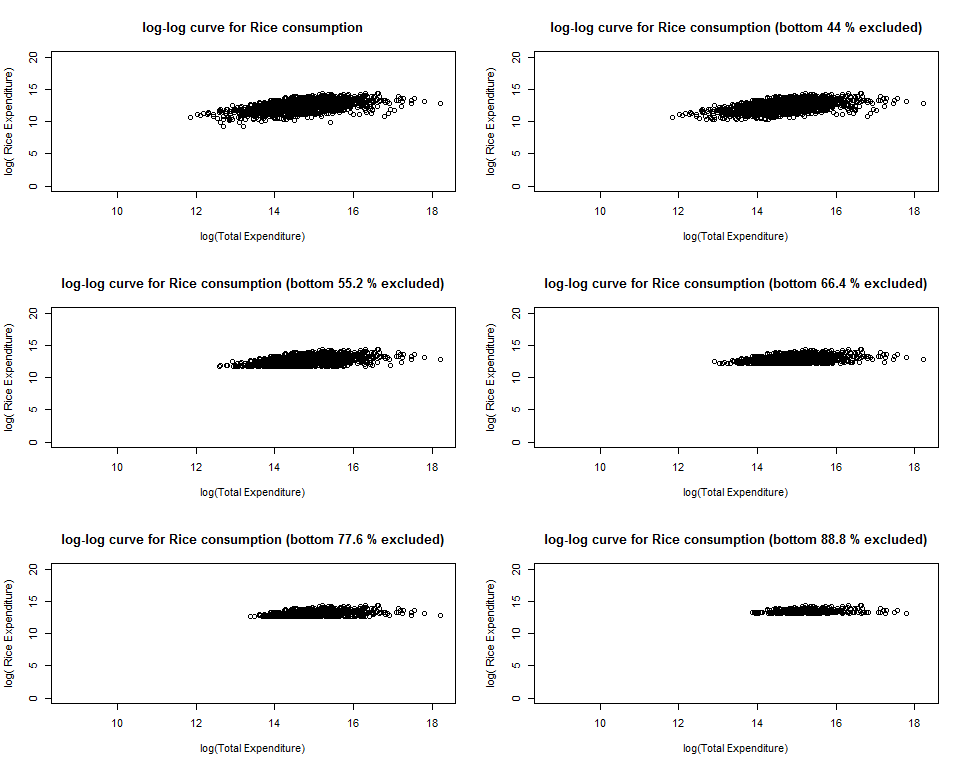
\includegraphics[scale=0.4]{lsms/loglogrice}
\par\end{centering}

\caption{LSMS Tazanania 2010: Percentiles of nonzero consumption of rice}
\end{figure}


\begin{figure}
\begin{centering}
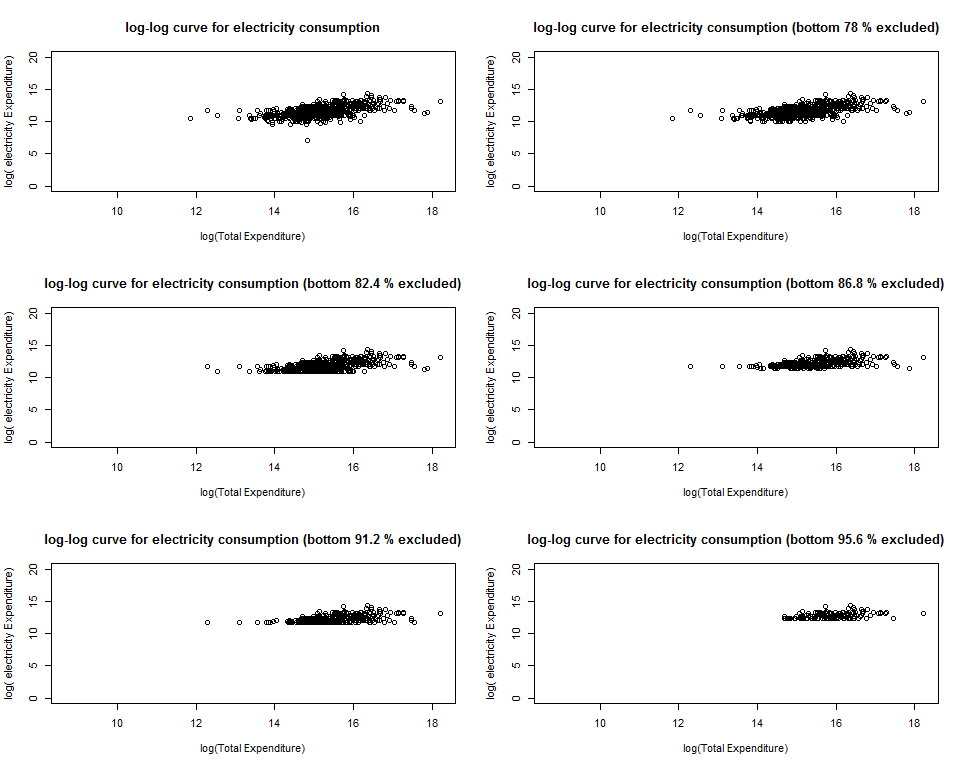
\includegraphics[scale=0.4]{lsms/loglogelectricity}
\par\end{centering}

\caption{LSMS Tazanania 2010: Percentiles of nonzero consumption of electricity}
\end{figure}


\begin{figure}
\begin{centering}
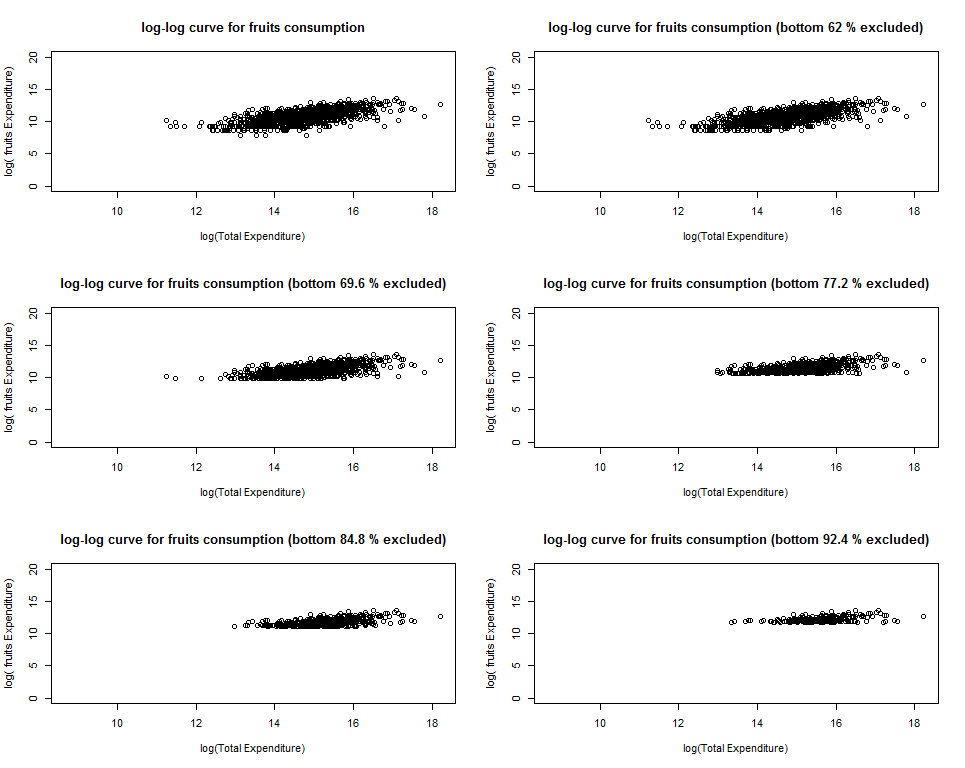
\includegraphics[scale=0.4]{lsms/loglogfruit}
\par\end{centering}

\caption{LSMS Tazanania 2010: Percentiles of nonzero consumption of fruits }
\end{figure}


\begin{figure}
\begin{centering}
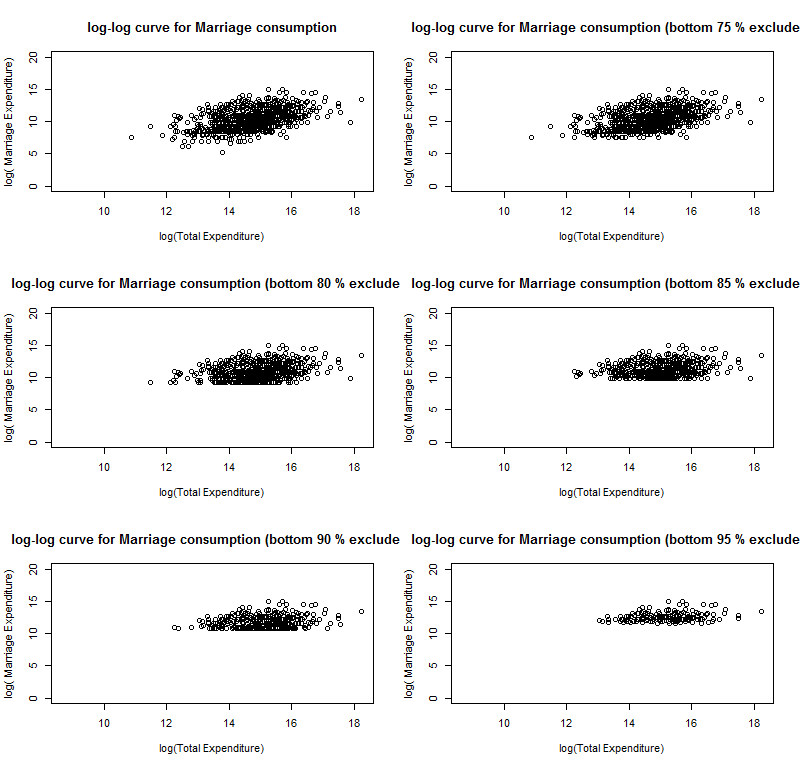
\includegraphics[scale=0.4]{lsms/loglogmarriage}
\par\end{centering}

\caption{LSMS Tazanania 2010: Percentiles of non-zero expenditure on marriage}
\end{figure}


\begin{figure}
\begin{centering}
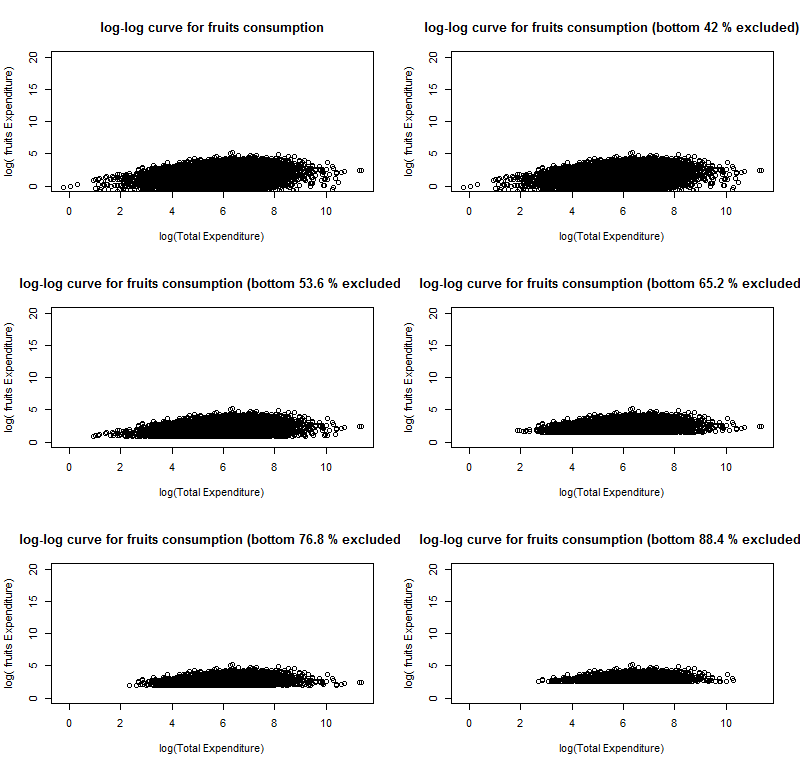
\includegraphics[scale=0.4]{cex/us_cex_fruits}
\par\end{centering}

\caption{US CEX (2004,2010,2014): Percentiles of non-zero consumption of fruits}
\end{figure}


\begin{figure}
\begin{centering}
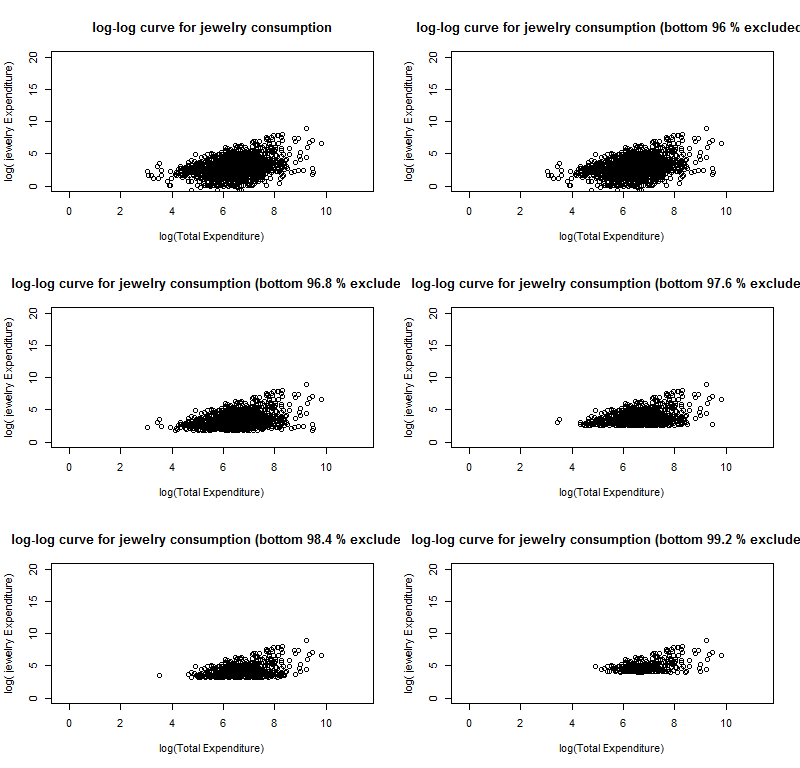
\includegraphics[scale=0.4]{cex/us_cex_jewelry}
\par\end{centering}

\caption{US CEX (2004,2010,2014): Percentiles of non-zero consumption of jewelry}
\end{figure}



\section{Analysis of LSMS Data}


\subsection{Steps in preparing LSMS data (2010)}

Following steps were performed before running the regressions on the
household consumption data from LSMS 2010\@.
\begin{enumerate}
\item Read weekly diary data from Section K (a table of items with the quantities
consumed and cost associated with the item for every household).

\begin{enumerate}
\item All items that had no cost assciated with them were \uline{ignored}
(not included in total consumption) 
\item Gift quantities were \uline{ignored} for consumption ( median ratio
of gift to total diary consumption was zero - only 132/3828 households
had this ratio 1\% or higher )
\item Weekly diary data was multiplied by 52 (to \uline{estimate} annual
consumption)

\begin{enumerate}
\item Weekly recall items were also multiplied by 52 (to \uline{estimate}
annual consumption)
\end{enumerate}
\item Monthly recall items were multiplied by 12 (to \uline{estimate}
annual consumption)
\item All expenditure from (c)-(e) above were summed up as total expenditure
\end{enumerate}
\item Obtained Personal Data from Section A,B,C and J files

\begin{enumerate}
\item Section C\_CB was read to obtain market facilitycode and gauge the
accessibility of a market in every district. The closest accessible
market could be either within the district or outside the district
at a given distance. If a market was within the the district or less
than \uline{10 kms away} it was deemed ``accessible''. Urban/rural
classifications based on population density could be inserted at this
stage (population density in not available in LSMS). 
\item Read section B and C files
\item Calculated age of member by subtracting YOB (year-of-birth) from 2010
(survey year) 
\item Read section J for housing data (total house rent, number of primary/secondary
rooms)
\end{enumerate}
\item Obtained income data from Section E (currently ignored for analysis
for it being sparse). Here, the recorded pay frequency was in hours,
days, weeks, months, fortnights, months, quarter, half year or year
- while the mandatory fields corresponding to all of these units were
i) number of hours worked per week ii) number of weeks worked per
month and iii) number of months worked in an year .

\begin{enumerate}
\item When pay was on a per-hour basis, the number of hours worked per week
(provided) was multiplied with the number of weeks worked per month
(provided). This product was then multiplied with the number of months
worked per year (provided) to estimate the annual income.
\item When pay was per-day, a \uline{10 hour working day} was assumed
to obtain the effective number of work-days per week (based on the
number of hours worked per week). This was then mutliplied with the
number of weeks worked per month in the year and then further multiplied
with the number of months worked in an year to obtain the estimated
annual income.
\item When pay was per week, the number of weeks worked per month was multiplied
with the number of months worked per year.
\item When pay was in fortnights, then twice the number of months worked
in an year was used to calculate the total income received over the
year.
\item When pay was per-month, then the multiplication factor was just the
number of months worked per year 
\item When pay was per-quarter, then the effective number of quarters were
inferred from the number of months worked per year (number\_of\_months/3)
and multiplied with the number of months worked per year to obtain
the estimated annual income.
\item For self-employed income, the work-months in an year was similarly
used to compute total income from self-employment in the year
\item All members less than 5 year old were \uline{ignored} from the
income data 
\item For wage workers:

\begin{enumerate}
\item summed up wages into column yearly pay 
\item summed up values under ``other forms of payment''
\item sum up values as secondary of payment (for wage-workers) 
\item only primary job was used to identify the employer type of the individual
\item added other wages from secondary job by summing up yearly-income from
all sources into the yearly income
\end{enumerate}
\end{enumerate}
\item Ignored bad data (outliers)

\begin{enumerate}
\item Ignored 5 households with exceedingly high expenditure on marriage
(more than reported annual income)
\item Ignored households in the income table but with zero income (number
of households with income data thus ignored were under 2\%)
\end{enumerate}
\item Merged all data

\begin{enumerate}
\item Set education expense of houses with education expenses= NA as zero
\item Summed up educational expense and total house rent from personal data
into total expenditure (both weren't a part of diary data)
\item Obtained personids of the house-heads and the following variables
for household-head: education-level, age, years in community, language,
occupation
\item Obtained visible expenditure by summing up expenditure on visible
items
\item Merged all data into one table
\end{enumerate}
\end{enumerate}

\subsection{Claims Tested}


\subsubsection{Effect of occupation}

Income data in LSMS is not available for all the surveyed households.
This may indicate the presence of informal sector in Tanzania. A few
occupations in the survey are neither well defined nor are truly an
indicator of total income. The presence of categories like unpaid-family-work
and of individuals with no-primary-job getting a significant income
from their secondary occupations makes the task of associating the
primary occupation of the household head with her income rather difficult
(i.e. occupation - which is available for all household heads cannot
be used as a proxy of household income - which is not available for
all households in the survey). Grouping the occupations into fewer
categories than in the survey (by putting paid/unpaid family work
and agriculture under the same category for example) allows for the
smoothening of the effect of individual occupations and may serve
as a proxy of socioeconomic classes in the country. Without or without
this grouping, the effect of occupation has been found significant
on the consumption of scarce commodities. The results are shown in
Table \ref{tab:no_instruments_reg1}.


\subsubsection{Effect of Education Level}

One of the claims to be evaluated on the LSMS data is whether education
has a significant effect on visible consumption. If the education
level of NA is considered as none (for nearly 30\% of the recorded
individuals), then highest education level of the household held is
found quite significant for many commodities.


\subsubsection{Effect of Immigration}

With a significant migration from rural areas, one of the claims to
be tested is whether those resident in the community spend less on
positional consumption. While this does seem be to be a significant
factor, it has a weaker effect than age or household size (which is
to be further split as number of children and the number of members
minus the number of children) .


\subsubsection{Urbanization Effects}

Most of Tanzania appears to be sparsely populated with little access
to basic services and it is likely that the administrative classifications
of rural-urban areas do not reflect the consumer markets so well.
Still, ``is\_rural'' dummy is found significant for house-rent and
electricity (since most of rural Tanzania does not have electricity
- See Table \ref{tab:no_instruments_reg1}). 

If one were to use a dummy for accessible markets (created using the
distance from the surveyed household location to the closest daily
market ) - the effect of such a dummy is not so significant on positional
consumption. The region dummies - on the other hand - are found to
have more significance - indicating regional disparities for conspicuous
consumption in the country.


\subsubsection{Population density}

Population density is a crude measure for crowding in the cities.
The regions with higher population density do have a slight effect
on consumption of scarce commodities. It is hoped that a urban/rural
dummy created by classifying districts based on their population densities
(or at a finer granularity than regional levels) may give a more detailed
view on the effect of population density on conspicuous consumption.


\subsubsection{Services as Visible Consumption}

One of the interesting observations in the Vindex survey (Heffetz\cite{heffetz_visibility})
is the clustering of services and products. It is found that services
tend to be less ``visible'' in the Western consumer world. The clustering
might not be as clear-cut in the developing world - where social stratification
is severe and many services are contractual (non-monetary). The socio-cultural
barriers might have an effect through access to services.

Towards that claim, English education as a control parameter is found
quite significant for positional consumption. Those who identify themselves
as English speakers tend to spend more on scarce commodities. This
indicates that English education may be quite scarce - and while it
isn't reflected in the consumer expenditure market data so easily
- it's likely to play a role in status competitions.

\begin{figure}
\centering{}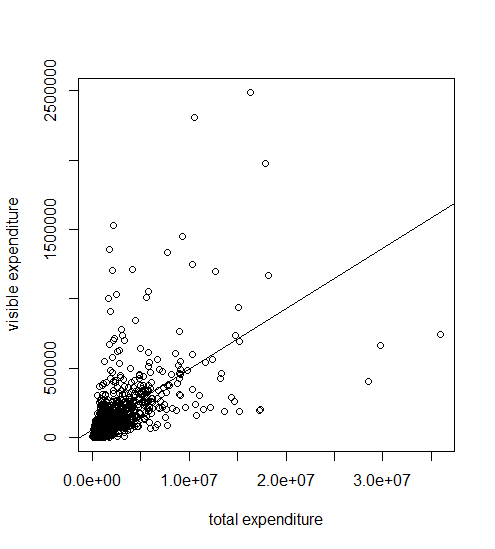
\includegraphics[scale=0.5]{lsms/lsms_visible_totexp_plot}\caption{Visible Expenditure vs Total Expenditure for LSMS 2010}
\end{figure}



\subsection{Analysis and Discussion}

Food is a significant portion of total spending overall \footnote{50\% of those surveyed spend 60\% or higher of their total expenditure
on food - subject to estimation errors.}. More importantly, those in non-agrarian professions spend about
as much of their total expenditure on food as those in agrarian occupations
\footnote{The median ratio of food-expenditure to total expenditure for agrarian
occupation households is 60\% while for non-agrarian occupations the
median is 57\%. Around 54\% of the total surveyed households were
in agrarian occupations.}. The other half of the expenditure is spent on housing, education
and energy requirements as well as various household products\footnote{Note that we may have slight errors in recording of food expenditure
due to extrapolation of the weekly diary}. 

While a commodity for private consumption (e.g. skin-cream or hobby-equipment
in the LSMS data) might have an appeal for everyone - whether it is
associated with high-income or not is a social psychological concern
and cannot be assessed from the household survey by itself. In the
absence of a visibility survey (asking the respondents how much they
notice a product and whether they associate the product with high-income
or not), one may still continue the discussion of the potential conspicuous
value of items by looking at how scarce the item is (based on the
percentile of consumers of the commodity). This is akin to repeating
the analysis of visible expenditure with a given commodity as the
only constituent of the visibility basket. The percentile of consumers
using a given commodity (e.g. top 22\% for electricity) and the slope
of $log(commodity-expenditure)$ vs $log(total-expenditure)$ can
tell us if richer sections of society spend more on a certain commodity
and if the poorer sections of society consume the chosen commodity
at all (the commodities chosen in the Table \ref{tab:regression_results}
are those where this slope is significant). The regression based on
data prepared from the last step attempts to calculate the coefficients
of the following equation:

\begin{equation}
ln(vis_{i})=\beta_{0}+\beta_{1}\cdot Dem_{i}+\beta_{2}\cdot ln(pInc_{i})+\epsilon\label{eq:lnvis_regression-2}
\end{equation}


Here $vis_{i}$ is the total visible consumption of the household
$i$ (expenditure on a chosen commodity such as electricity, sports
equipment), $Dem_{i}$ is a vector of demographic indicators under
consideration and $pInc_{i}$ is the permanent income - proxied by
total expenditure - which has been instrumented using $age$, $cubic(age)$,
$occupation$, $highest\_education$ level , $ln(highest\_education)$,
$cubic(highest\_education)$ \footnote{All 2sls regressions involved involved performing three diagnostic
tests provided by the function ivreg of package AER in R. These tests
are - i) a weak instrument test ii) a Wu-Hausman test for endogeneity
and iii) a Sargan test for validity of instruments.}.

Table \ref{tab:regression_results},\ref{tab:no_instruments_reg1}
and \ref{tab:instrumented_reg1}summarize the results obtained by
running regressions on several commodity-categories. A column in the
Table \ref{tab:regression_results} also suggests the percentile of
consumers using the commodity (electricity for example is used amongst
those having top 22\% of total expenditure). The usage of commodities
such as skincream and other-personal-products (shampoos, razors etc.)
are widespread compared with sports or hobby equipment and electricity.
For commodities that are rare and consumed only amongst the richer
sections of the society (those with higher total expenditure) the
effect of English literacy is significant. Similarly, hsize has a
significant effect on both educational expense and personal products
(using number of children instead of hsize could provide better association
with education expense).

We cannot claim from the results that the population spends more on
status commodities than education. What we can claim however, is that
electricity is more scarce than education. Further, in areas where
food is expensive, spending on marriage reduces - particularly by
the occupations that may bring higher incomes. This marks a preference
towards industrial goods in the urban (expensive) areas.

Another observation that can possibly help in modeling scarcity is
that scarcity of items seems to occur in clusters of objects. Carpets-rugs
require a certain housing status and access to English depends on
region. Similarly, many hobby equipments may require access to electricity
etc. The clustering of these items essentially point to the urban-rural
differences in the country.

\begin{table}
\centering{}%
\begin{tabular}{|>{\raggedright}p{4cm}||>{\raggedright}p{4cm}||>{\raggedright}p{2cm}||>{\raggedright}p{4cm}|}
\hline 
\multirow{1}{4cm}{Commodity} & Significant Variables & NonConsumer Percentile  & Variables significant after lnpinc instrumentation\tabularnewline
\hline 
\hline 
\multirow{1}{4cm}{carpetsrugs} & lnpinc, age, hsize, housingstatus, highest\_educ, english & 78 & lnpinc, age,hsize,

highest\_educ,

english\tabularnewline
\hline 
\hline 
educexpense & lnpinc, age, hsize, housingstatus, occupation & 35 & lnpinc,age,

hsize,

housingstatus,

occupation\tabularnewline
\hline 
\hline 
electricity & lnpinc, age, hsize, housingstatus, occupation, isrural, highest\_educ,
region, english, is\_resident & 78 & Chosen instruments (occupation, ln\_highest\_educ ) 

did not demonstrate endogeneity of lnpinc\tabularnewline
\hline 
\hline 
houserent & lnpinc, age, housingstatus, roomsnum & 84 & lnpinc,

housingstatus\tabularnewline
\hline 
\hline 
personal items repair & lnpinc, highest\_educ, region & 96 & lnpinc, highest\_educ, region\tabularnewline
\hline 
\hline 
personal products & lnpinc, hsize, roomsnum, years\_community & 37 & lnpinc, hsize, roomsnum, years\_community\tabularnewline
\hline 
\hline 
skin cream & lnpinc, age, hsize, isrural, region, years\_community & 12 & lnpinc, age, hsize, region, years\_community\tabularnewline
\hline 
\hline 
funeral costs & lnpinc, region, roomsnum & 54 & lnpinc, region, roomsnum\tabularnewline
\hline 
\hline 
marriage costs & lnpinc, region, english, roomsnum, years\_community & 75 & lnpinc, region, english, roomsnum, years\_community\tabularnewline
\hline 
\hline 
sports and hobby equipment & lnpinc, age, housingstatus, region, english & 93 & lnpinc, age, housingstatus, region, english\tabularnewline
\hline 
\end{tabular}\caption{\label{tab:regression_results}Results from regression over selected
variables}
\end{table}

\begin{landscape}
\begin{table}
[!htbp] \centering 
\caption{\label{tab:no_instruments_reg1} Regression for scarce commodities with no instrumentation}
\resizebox{\columnwidth}{!}{
\begin{tabular}{@{\extracolsep{5pt}}lcccccccccc} 
\\[-1.8ex]\hline 
\hline \\[-1.8ex] 
 & \multicolumn{10}{c}{\textit{Dependent variable: consumption}} \\ 
\cline{2-11} 
\\[-1.8ex] & \multicolumn{10}{c}{depvar} \\ 
\\[-1.8ex] & carpetsrugs(1) & education(2) & electricity(3) & houserent(4) & personalitemsrepair(5) & personalprods(6) & skincream(7) & funeral(8) & marriage(9) & hobbyequipment(10)\\ 
\hline \\[-1.8ex] 
 lnpinc & 4.708$^{***}$ & 3.574$^{***}$ & 4.391$^{***}$ & 1.154$^{***}$ & 0.843$^{***}$ & 3.439$^{***}$ & 2.145$^{***}$ & 2.759$^{***}$ & 3.296$^{***}$ & 1.214$^{***}$ \\ 
  & (0.328) & (0.239) & (0.332) & (0.173) & (0.170) & (0.281) & (0.207) & (0.260) & (0.261) & (0.142) \\ 
  & & & & & & & & & & \\ 
 age & $-$0.106$^{***}$ & 0.086$^{***}$ & 0.067$^{***}$ & $-$0.067$^{***}$ &  &  & $-$0.042$^{***}$ &  &  & $-$0.038$^{***}$ \\ 
  & (0.023) & (0.017) & (0.020) & (0.011) &  &  & (0.015) &  &  & (0.010) \\ 
  & & & & & & & & & & \\ 
 hsize & $-$0.459$^{***}$ & 2.160$^{***}$ & $-$0.529$^{***}$ &  &  & $-$0.506$^{***}$ & 0.217$^{***}$ &  &  &  \\ 
  & (0.115) & (0.089) & (0.102) &  &  & (0.104) & (0.067) &  &  &  \\ 
  & & & & & & & & & & \\ 
 housingstatus & 0.600$^{***}$ & $-$1.049$^{***}$ & 0.924$^{***}$ & 4.280$^{***}$ &  &  &  &  &  & 0.452$^{***}$ \\ 
  & (0.208) & (0.187) & (0.191) & (0.131) &  &  &  &  &  & (0.106) \\ 
  & & & & & & & & & & \\ 
 occupation\_rank &  &  & 0.782$^{***}$ &  &  &  &  &  &  &  \\ 
  &  &  & (0.295) &  &  &  &  &  &  &  \\ 
  & & & & & & & & & & \\ 
 isrural &  &  & $-$6.468$^{***}$ & $-$3.501$^{***}$ &  &  & 1.469$^{***}$ &  &  &  \\ 
  &  &  & (0.642) & (0.419) &  &  & (0.465) &  &  &  \\ 
  & & & & & & & & & & \\ 
 highest\_educ & $-$0.295$^{***}$ &  & 0.421$^{***}$ &  & 0.075$^{**}$ &  &  &  &  &  \\ 
  & (0.076) &  & (0.066) &  & (0.035) &  &  &  &  &  \\ 
  & & & & & & & & & & \\ 
 region &  &  & 0.186$^{***}$ & $-$0.051$^{***}$ & $-$0.049$^{***}$ &  & $-$0.121$^{***}$ & $-$0.142$^{***}$ & $-$0.034$^{**}$ & $-$0.066$^{***}$ \\ 
  &  &  & (0.017) & (0.011) & (0.010) &  & (0.012) & (0.018) & (0.016) & (0.009) \\ 
  & & & & & & & & & & \\ 
 english & 3.146$^{***}$ &  & 2.949$^{***}$ &  &  &  &  &  & 1.976$^{**}$ & 1.633$^{***}$ \\ 
  & (0.953) &  & (0.840) &  &  &  &  &  & (0.794) & (0.455) \\ 
  & & & & & & & & & & \\ 
 roomsnum &  &  &  & $-$0.919$^{***}$ &  & 0.442$^{***}$ &  & 0.625$^{***}$ & 0.654$^{***}$ &  \\ 
  &  &  &  & (0.100) &  & (0.169) &  & (0.157) & (0.146) &  \\ 
  & & & & & & & & & & \\ 
 is\_resident &  &  & $-$1.956$^{***}$ & $-$1.977$^{***}$ &  &  &  &  &  &  \\ 
  &  &  & (0.558) & (0.366) &  &  &  &  &  &  \\ 
  & & & & & & & & & & \\ 
 years\_community &  &  &  &  &  & $-$0.073$^{***}$ & $-$0.026$^{**}$ &  & $-$0.054$^{***}$ &  \\ 
  &  &  &  &  &  & (0.015) & (0.013) &  & (0.014) &  \\ 
  & & & & & & & & & & \\ 
 Constant & $-$71.251$^{***}$ & $-$64.314$^{***}$ & $-$85.424$^{***}$ & $-$31.269$^{***}$ & $-$33.945$^{***}$ & $-$47.620$^{***}$ & $-$21.851$^{***}$ & $-$46.797$^{***}$ & $-$61.169$^{***}$ & $-$36.167$^{***}$ \\ 
  & (4.287) & (3.438) & (4.610) & (2.689) & (2.214) & (4.026) & (3.020) & (3.654) & (3.767) & (2.098) \\ 
  & & & & & & & & & & \\ 
\hline \\[-1.8ex] 
Observations & 2,240 & 2,965 & 2,240 & 2,965 & 2,240 & 2,965 & 2,965 & 2,965 & 2,963 & 2,963 \\ 
R$^{2}$ & 0.126 & 0.322 & 0.437 & 0.502 & 0.029 & 0.084 & 0.094 & 0.059 & 0.101 & 0.073 \\ 
Adjusted R$^{2}$ & 0.124 & 0.321 & 0.435 & 0.501 & 0.027 & 0.082 & 0.092 & 0.058 & 0.100 & 0.071 \\ 
Residual Std. Error & 13.394 (df = 2233) & 13.463 (df = 2960) & 11.595 (df = 2229) & 8.929 (df = 2957) & 7.386 (df = 2236) & 14.919 (df = 2960) & 10.078 (df = 2958) & 15.518 (df = 2961) & 13.840 (df = 2957) & 7.963 (df = 2957) \\ 
F Statistic & 53.824$^{***}$ (df = 6; 2233) & 351.136$^{***}$ (df = 4; 2960) & 173.281$^{***}$ (df = 10; 2229) & 426.503$^{***}$ (df = 7; 2957) & 21.953$^{***}$ (df = 3; 2236) & 67.429$^{***}$ (df = 4; 2960) & 51.003$^{***}$ (df = 6; 2958) & 61.522$^{***}$ (df = 3; 2961) & 66.629$^{***}$ (df = 5; 2957) & 46.343$^{***}$ (df = 5; 2957) \\ 
\hline 
\hline \\[-1.8ex] 
\textit{Note:}  & \multicolumn{10}{r}{$^{*}$p$<$0.1; $^{**}$p$<$0.05; $^{***}$p$<$0.01} \\ 
\end{tabular} 
}
\end{table}
\end{landscape}


\begin{landscape}
\begin{table}
[!htbp] \centering
\caption{\label{tab:instrumented_reg1}Instrumented Regression for scarce commodities}
\resizebox{\columnwidth}{!}{
\begin{tabular}{@{\extracolsep{5pt}}lcccccccccc} 
\\[-1.8ex]\hline 
\hline \\[-1.8ex] 
 & \multicolumn{10}{c}{\textit{Dependent variable:}} \\ 
\cline{2-11} 
\\[-1.8ex] & lnvis & lndseducexpense & lnvis & lndshouserent & \multicolumn{6}{c}{lnvis} \\ 
\\[-1.8ex] & carpetsrugs(1) & education(2) & electricity(3) & houserent(4) & personalitemsrepair(5) & personalprods(6) & skincream(7) & funeral(8) & marriage(9) & hobbyequipment(10)\\ 
\hline \\[-1.8ex] 
 lnpinc & 4.665$^{***}$ & 3.033$^{***}$ & 9.941$^{***}$ & 0.982$^{**}$ & 0.747$^{**}$ & 3.216$^{***}$ & 1.661$^{***}$ & 2.770$^{***}$ & 3.446$^{***}$ & 1.593$^{***}$ \\ 
  & (0.657) & (0.597) & (1.247) & (0.432) & (0.321) & (0.565) & (0.502) & (0.484) & (0.627) & (0.318) \\ 
  & & & & & & & & & & \\ 
 age & $-$0.106$^{***}$ & 0.081$^{***}$ & 0.055$^{***}$ & $-$0.074$^{***}$ &  &  & $-$0.040$^{**}$ &  &  & $-$0.060$^{***}$ \\ 
  & (0.023) & (0.017) & (0.021) & (0.016) &  &  & (0.020) &  &  & (0.014) \\ 
  & & & & & & & & & & \\ 
 hsize & $-$0.454$^{***}$ & 2.227$^{***}$ & $-$1.182$^{***}$ &  &  & $-$0.518$^{***}$ & 0.346$^{***}$ &  &  &  \\ 
  & (0.131) & (0.112) & (0.178) &  &  & (0.140) & (0.099) &  &  &  \\ 
  & & & & & & & & & & \\ 
 housingstatus & 0.605$^{***}$ & $-$0.979$^{***}$ & 1.028$^{***}$ & 4.402$^{***}$ &  &  &  &  &  & 0.491$^{***}$ \\ 
  & (0.217) & (0.200) & (0.203) & (0.157) &  &  &  &  &  & (0.127) \\ 
  & & & & & & & & & & \\ 
 occupation\_rank &  &  & $-$0.723 &  &  &  &  &  &  &  \\ 
  &  &  & (0.451) &  &  &  &  &  &  &  \\ 
  & & & & & & & & & & \\ 
 isrural &  &  & $-$3.861$^{***}$ & $-$3.618$^{***}$ &  &  & 0.951 &  &  &  \\ 
  &  &  & (0.883) & (0.585) &  &  & (0.626) &  &  &  \\ 
  & & & & & & & & & & \\ 
 highest\_educ & $-$0.292$^{***}$ &  & 0.132 &  & 0.084$^{*}$ &  &  &  &  &  \\ 
  & (0.089) &  & (0.094) &  & (0.044) &  &  &  &  &  \\ 
  & & & & & & & & & & \\ 
 region &  &  & 0.187$^{***}$ & $-$0.057$^{***}$ & $-$0.049$^{***}$ &  & $-$0.106$^{***}$ & $-$0.138$^{***}$ & $-$0.054$^{***}$ & $-$0.076$^{***}$ \\ 
  &  &  & (0.018) & (0.014) & (0.010) &  & (0.014) & (0.021) & (0.020) & (0.012) \\ 
  & & & & & & & & & & \\ 
 english & 3.155$^{***}$ &  & 2.263$^{**}$ &  &  &  &  &  & 2.253$^{**}$ & 1.574$^{***}$ \\ 
  & (0.962) &  & (0.903) &  &  &  &  &  & (0.984) & (0.577) \\ 
  & & & & & & & & & & \\ 
 roomsnum &  &  &  & $-$1.020$^{***}$ &  & 0.589$^{***}$ &  & 0.412$^{**}$ & 0.518$^{***}$ &  \\ 
  &  &  &  & (0.132) &  & (0.197) &  & (0.186) & (0.183) &  \\ 
  & & & & & & & & & & \\ 
 is\_resident &  &  & $-$0.369 & $-$2.191$^{***}$ &  &  &  &  &  &  \\ 
  &  &  & (0.684) & (0.494) &  &  &  &  &  &  \\ 
  & & & & & & & & & & \\ 
 years\_community &  &  &  &  &  & $-$0.077$^{***}$ & $-$0.033$^{*}$ &  & $-$0.065$^{***}$ &  \\ 
  &  &  &  &  &  & (0.020) & (0.017) &  & (0.020) &  \\ 
  & & & & & & & & & & \\ 
 Constant & $-$70.746$^{***}$ & $-$56.921$^{***}$ & $-$156.675$^{***}$ & $-$28.337$^{***}$ & $-$32.733$^{***}$ & $-$44.482$^{***}$ & $-$15.511$^{**}$ & $-$46.113$^{***}$ & $-$62.420$^{***}$ & $-$40.656$^{***}$ \\ 
  & (7.971) & (8.229) & (16.113) & (6.362) & (4.088) & (8.068) & (7.060) & (6.874) & (9.036) & (4.486) \\ 
  & & & & & & & & & & \\ 
\hline \\[-1.8ex] 
Observations & 2,240 & 2,965 & 2,240 & 2,240 & 2,240 & 2,240 & 2,240 & 2,240 & 2,240 & 2,240 \\ 
R$^{2}$ & 0.126 & 0.321 & 0.367 & 0.502 & 0.028 & 0.069 & 0.080 & 0.043 & 0.090 & 0.078 \\ 
Adjusted R$^{2}$ & 0.124 & 0.320 & 0.364 & 0.500 & 0.027 & 0.067 & 0.077 & 0.042 & 0.088 & 0.076 \\ 
Residual Std. Error & 13.394 (df = 2233) & 13.474 (df = 2960) & 12.299 (df = 2229) & 9.500 (df = 2232) & 7.386 (df = 2236) & 14.768 (df = 2235) & 9.766 (df = 2233) & 15.740 (df = 2236) & 14.286 (df = 2234) & 8.484 (df = 2234) \\ 
\hline 
\hline \\[-1.8ex] 
\textit{Note:}  & \multicolumn{10}{r}{$^{*}$p$<$0.1; $^{**}$p$<$0.05; $^{***}$p$<$0.01} \\ 
\end{tabular}
}
\end{table}
\end{landscape}


\part{A Behavioural Model for Status Utility}


\section{A model for Utility and Status}

The concept of status is rather non-trivial and has characteristics
of a feedback system in the long-run (status may yield income through
social barriers but requires income to be acquired). The Ireland model
used in the literature treats status-signaling as purchasing of visible
and non-visible goods\cite{ireland_signals}. In the Ireland model,
the combined utility for every consumer is $U=F(f(v,w),s)$ where
$f(v,w)$ is the private utility of the consumer and status $s$ is
assumed to be an increasing function of inference of others - $s=f(v,g(v)$)
- with $v$ denoting visual consumption and $w$ - the consumption
that is not directly observable. Every consumer thus optimizes the
combined private and visible utility. A practical consideration in
the model is the separation between visible and non-visible consumption
- a boundary that requires a socio-culutral judgment and has been
drawn using consumer surveys in the literature.

What research in the developing markets further points out is that
the parameter of combined utility in a simplified model - ($U=(1-a)\cdot f(v,w)+a\cdot f(v,g(v)$)
- can vary for different sections of society. A slight adjustment
of the model may be to add another parameter that indicates the consumer's
social class. This may be relevant in the developing world where social
status is yielded through social barriers. Sections of society that
are endowed with a higher status capital may be in less of a need
to purchase commodities of visible consumption.

In the analysis of LSMS data on Tanzania so far, urban/rural differences
have significance in the consumption of scarce commodities. There
are two ways to incorporate this into a model of signaling - one is
to consider these household characteristics as a social class of consumers
so that different visible sensitivities for social classes is noted.
The other is to consider these characteristics as part of conspicious
consumption in the long-run. For example, English literacy seems to
have correlation with the consumption of certain scarce products in
Tanzania. In the model of scarcity, English literacy (along with urban
residence and other characteristics significant for consumption of
scarce commodities) would be seen as a status commodity (capital)
that is acquired through spending on education or migration (or other
relevant commodities).


\subsection{A Word of Caution}

Notice that one needs to be careful while drawing conclusions based
on consumption of commodities that are themselves selected based on
the percentiles of consumption levels. The threshold method that we
use to select scarce commodities (that are likely to be visible) -
considers items that i) are accessible by no more than 50\% of the
consumers and ii) have their expenditure rising with permanent income.
These are - by definition - items that the rich are more likely to
afford. We cannot select items that the only richer section of society
indulges in and claim that people spending on these selected items
indicate higher status. Such a claim is only a restatement of the
high permanent income and says nothing more substantial than that
the richer population sections signal higher status. It would be a
fallacy to associate visible consumption with household characteristics
by only associating household characteristics with permanent income.
The threshold method that we use only measures the ``scarcity''
of the item (e.g. electricity is more scarce than food) - not status
or visibility per se - which involve some socio-cultural judgement.
That scarcity itself has an indirect effect on status competitions
cannot be denied - but this effect is not measured by the threshold
method of classifying alone.


\section{A model for scarcity and congestion}

In recent decades, the urban settlements in Africa have seen massive
overpopulation and development of the services sector. The differences
in urban-rural lifestyles have increased. The scarcity of services
and of industrial goods (which would be a necessity in the Western
world) seem evidently sparse in the developing countries (a claim
that is verified by data on Tanzania).

A relevant question amidst these developments is whether a consumer
prefers a larger house over installation of electricity or not. As
a commodity, electricity is both scarce and visible - as it opens
up more lifestyle choices. A survey detailed in the next sections
aims to test the presence of a preference for electricty (and other
scarce goods) - but as is, the data suggests significant urban-rural
differences across regions in Tanzania. In a Hirschian sense, a congestion
\cite{HirschSocialLimits} is likely to exist for electricity. 

A general view on scarcity would allow us to classify the commodities
based on their scarcity and quantify the urban-rural differences better.
The survey detailed in next sections may further help measure the
impact of such scarcities on consumer preferences. It is noted that
many of the items are scarce together (carpets and housing-status,
electricty and hobby equipments, etc.) . It is through such denial
of goods and services that status perceptions develop. A simple view
of observed scarcities can be provided by a directed graph of items
for classification - where a node is an item and points to other nodes/items
that it denies (which themselves can be formed with items that deny
other items and so and so forth). For example, electricity can be
a node in this graph with connections to equipments and electronics
but no connection to food items. The disconnected nodes in the graph
- would be least likely to be affected by another unreachable node
in the graph. The criteria of connections (denials) would be determined
by statistical significance e.g. rice and walnuts appear would not
be scarce together if one of them is available and affordable by both
higher and lower quantiles of permanent income of society.


\section{A Behavioural Experiment for Status Competitions}


\subsection{Status and Consumption as games}

Behavioural games have been used in the developing countries to gauge
motivations of the participating consumers \footnote{A study by Sophie Clot studies the effect high and low effort work
on consumption by conducting an experiment at the payment office where
some amount of pay is distributed for low-effort work and some for
high-effort work.}. While the visibility surveys (\cite{ZahraIndia,heffetz_visibility})
attempt to study how consumption on certain commodities may signal
status, the goal of the proposed game is to characterise environments
under which the perceptions of a higher-status may develop. The game
attempts to emulate i) the consumer market and ii) the mechanism through
which status may be assigned within a group of consumers. It therefore
relies on participants playing the dual role of a consumer and status-observer.

The activities of purchasing and assigning status are separate in
the game. Since a simulated purchase performed by the participants
in the game (given a list of commodities, prices and outlay) is quite
likely to deviate from their real world purchases and their real needs,
the participants are instead asked what additional items they would
purchase for a given a basket of commodities that they already possess
(using a cumulative voting scheme that emulates selection of commodities
in a market - see section \ref{sub:Purchasing_Mechanism} for details).
The second part of the game emulates status assignment - where participants
assign a score of status and effectiveness each to 3 (or more) other
participants in the game by looking at the quantities of the item
categories possessed and purchased by the latter. The judgment of
status in the real world does not involve direct observance of prices
and thus it is only the quantity of the identified items consumed
or already possessed that matters in the status-assignment part of
the game. The end-goal of the game is to purchase a basket most desired
by others - the winner achieves this goal by purchasing commodities
of her choice that are most desirable by everyone and are indicative
of a rank higher than everyone else in the game.


\subsection{\label{sub:Purchasing_Mechanism}Purchasing Mechanism}

It is difficult for players to conduct a ``simulated shopping''
in a way that truly represents their needs. Hence, instead of asking
the respondent how they'll spend the given outlay of a 1000 dollars
over a set of commodities, they are asked how they would spend the
additional 100 dollars for a given 1000 dollars of outlay (or more)
value of items that they already have stocked up. The ``stock''
items can be chosen by the players as a first step in the game and
is intended to match their own consumption pattern. While the ``stock''
is made of non-positional items, the participants choose 3 items from
a mix of non-positional items and positional items - given the 10\%
extra outlay. Since all participants cannot be assumed to be equally
numerate, the game uses a scheme similar to cumulative voting - where
10 virtual coins are provided to the participant and the participant
is asked to distribute the coins amongst a set of available items
(both positional and non-positional). The provided outlay in the game
(number of coins) may vary for participants - in proportion to the
income distribution that is observed in the relevant consumption surveys
(e.g. LSMS for Tanzania).

In summary the following steps are taken in the game:
\begin{enumerate}
\item \label{enu:step_stock}Choose a stock basket that is closest to one's
own consumption pattern (no more than 5 basket classifications are
provided to choose from)
\item Acknowledge the real-life constraint (see Section \ref{sub:constraints})
\item Use the given additional outlay (10 or less virtual coins) to purchase
and add (positional and well as non-positional items) to the strictly
non-positional stock basket that was selected in the step \ref{enu:step_stock}\footnote{It is necessary to estimate the price of products and services for
the purchasing game to emulate the market.}
\item Provide a score (1..5) on effectiveness and status to 3 other participants
whose total outlay and the choice of items purchased (along with number
of coins used for every item) is also known
\end{enumerate}

\subsubsection{\label{sub:basket_mixes}Mixes in the Consumer Basket}

While the basket for every consumer can be varied to model urban/rural
differences or the distance /accessibility of the particular commodity
classes, the game ensures that all participants have reasonably similar
consumer universe. Consequently, no category is intended to be completely
removed from the basket (i.e. all baskets have the same set of categories).
Following are the categories for which the positional/non-positional
variants are sought:
\begin{enumerate}
\item Food - Fruits, Meat, Baked Goods or Nuts/Cereals and Pulses, Milk
(minor items such as salt and spices are not included), Tea, Soda/
Beer and Wine
\item Household products (Detergent, Electronics)
\item Personal Products (Clothes, Shoes, Makeup)
\item Household services (House refurbishments) and Energy (electricity/kerosene)
\item Savings for future Asset purchase
\item Entertainment/Dining Out/Travel/Travel Abroad
\item Health
\item Education (School/University)
\end{enumerate}

\subsubsection{\label{sub:constraints}Constraints and Assets}

The game attempts to measure status and consumption with respect to
high asset ownership, social class or familial responsibility. Since
players choose between physical needs and positional needs in the
game, a different circumstance is likely to affect their choice and
hence their perceived status. The game presents a precondition to
the player - indicating high asset ownership, a chosen social class
or a familial liability. For example, to test a participant's choice
between food and electricity, the game can present a large family
as a constraint, and record the choice between spending more on food
vs installing electricity. The game thus measures indirect effects
of reward or constraints on status by allowing participants to gauge
the suitability of a participant's choice in the status game in the
presence of constraints (familial) or rewards (asset-related).

Notice that the constraint variable is only planned to be binary in
the current scheme i.e. it is either a reward or a liability (when
present). The two values are expected to have an opposite affect on
the purchase of new items. Admittedly, the binary values of constraints
vs rewards circumvent the difficulty in comparisons between disparate
needs of the consumers - e.g. a large family, senior member or a social
event (e.g. marriage/funeral). While a multivalued variable (if adopted)
can potentially provide better insights into the relative effects
of these several types constraints, the goal of the current exercise
is to test for a direct effect of constraints on status (rather than
relative effect of the various possible constraints).


\subsection{Status ranking}

The status-ranking activity involves a student assigning a status
score by looking at i) what the other participant with a given income
level does with the extra outlay and ii) what the participant already
possesses. In the ranking scheme, the participants provide a score
on effectiveness as well as status to all the other (3 or more) participants
observed. Notice that in presence of constraints specified in section
\ref{sub:constraints}, regardless of whether one is selfish or not,
a participant would tend to penalise someone else who she thinks is
going to be more selfish than herself. Since the game provides a way
to penalize selfishness by status ranks, the participants are discouraged
from indicating status through overspending on positional items. The
penalty for not caring for a sick parent may be huge in the society
but so can be the penalty for being stingy. Similarly, while some
may want to indicate wealth by buying a watch they may also fear disrespect
for not taking care of a sick family member. The scores on effectiveness
and status are thus not only a way to discourage the consumer from
limiting the unrealistic purchases in the simulated purchasing part
of the game, they also track the effect of the externalities such
as sickness or age (measured through the binary variable discussed
in section \ref{sub:constraints}).

While consumers try to maximise their utility by purchasing more items
for a given limited outlay - they also manage their prestige by letting
others have a better opinion of themselves. The status game can thus
be seen as an enhanced version of the survey that asks people to imagine
a neighbour who spends more than them on a chosen commodity (used
in \cite{ZahraIndia,heffetz_visibility}). The proposed game attempts
to measure how consumers might act given a certain circumstances while
both status and welfare (effectiveness score can be seen as a proxy
of concern for others) become part of the payoff function in the game. 


\subsection{Welfare and Status competitions}

The solution of this game for a set of rational players remains a
pending exercise in this study. The key motivation for the analysis
at this point is that fundamentally all social welfare concerns are
concerns of Pareto optimality. Moreover, the payoff function for effectiveness
in the game is meant to be a proxy for welfare. 

With Pareto optimality in mind, more spending on education, health
seems desirable - but it may be become distant for consumers due to
their immediate needs - whether positional or non-positional. A comparison
with what is observed in consumption data versus what is observed
about positional consumption in games can provide some insight into
the social status that can influence the desired welfare equilibrium.


\subsection{Survey Questionnaire}

You have 10,000 (or 100) to spend today. What are the objects that
you would purchase if you were to enter the market today? Please take
a look at the constraints that might affect your consumption. Try
choosing the smartest way possible - the prices. You would also need
to compare 2 other candidates as part of this game (as others would
rate you). Try being close to your real circumstances. Unrealistic
values may disqualify you from the game.


\section{\label{sec:status_consumption_need}Policy implications}

The discussion so far leans towards permitting status competitions
rather than attempting to tax or control them. This is in line with
the suggestions offered by Robert H Frank \cite{FrankPond} favouring
a non-monetary market of stauses only so that status games (which
are a necessity) do not overlap with the market for real goods. Due
to structural reasons of the modern economy, advertising efforts can
turn a social scarcity into a physical scarcity (to use the Hirsch's
terminology\cite{HirschSocialLimits}). A profit-driven industry and
the advertising pursued by the companies tend to increase the status
competition for a commodity. Instead of letting status competitions
modify the distribution of that physical goods through competition
(and thus do little to avoid the problem of physical scrarcities in
the developing countries), policy can attempt to provide status-games
in a world of non-necessity items - in some ways to diffuse the status
competitions in the society.

In poor and non-pecuniary societies, the desire to become rich or
the benefit of inheriting money and education is often less reachable.
Status and money translate into social securities in unstructured
societies. These may well be detected in the countries in Africa -
but limited data on household characteristics in Tanzania (related
to ethnicity or religion) have prevented us from such an analysis
for Tanzania.

The question that we seek the answer for in the context of Tanzania
(or another developing country) is whether the expenditure on high-status
or scarce items (an analysis similar to one conducted by Prais Houthakker
for expensive and cheap tea varieties amongst social classes in the
UK\cite{HouthakkerFamilySurvey}) - is actually more desirable than
on housing and education. The designed experiment intends to find
answer to this question. If the answer is indeed the former, then
it makes sense to limit the status competitions through policy to
support status competitions on non-essential items (possibly by introducing
brand differentiation). Attaching glamour to education, healthcare
and food items may help consumers prioritize their needs.


\part{Effect of Price on food vs non-food items}


\section{Price Changes}

The literature has not used panel data analysis in the context of
conspicuous consumption. While an influence of rising prices can complicate
the analysis of visible consumption indicators, the insights from
demand elasticities are essential to understanding the relative effect
of status-related consumption against other commodities. Higher price
of food items may suppress consumption on food - but one cannot answer
whether an increase in price of food suppresses its consumption more
than it suppresses consumption of non-food items or not - without
an estimation of demand elasticities. Such details of consumption
patterns are basket-dependent and are not accessible without a record
of prices of all types of items in the basket. Unfortunately, a lack
of prices for non-food items in the LSMS prevent this much desired
time-series analysis.

Even though an analysis on non-food prices is inaccessbile with the
unavailability of price data in most consumption surveys (e.g. LSMS),
a time-series analysis based on food prices alone can provide insights
into the pressures on food consumption. Using historical prices on
calorie consumption in India, Deaton and Jean Dreze point out that
the overall calorie consumption has declined while the total outlay
has increased in India (\cite{DeatonDrezeIndiaFood}). The change
in positional value of food - determined by price differentiation
in the market and scarcity - can potentially help explain some of
this decline. While such a decline is reported to be less in the case
of sub-Saharan African countries than in India, the regional differences
within the country could be explained by the change of food's position
in the consumer universe (i.e. the so-called ``Sen argument''\cite{DeatonDrezeIndiaFood}).

Congestion - a related phenomenon - is subject to demand and supply
for a particular commodity and can be measured. If we were to consider
food, for example, a limited supply and overpopulation can increase
competition. Similarly, for entertainment, censorship and introduction
of internet can create new competitions (congestion). For housing,
new constructions and overpopulation can cause congestion. These are
commodity-specific instances and a focus on selected items may be
the only way to test whether the changes in consumption patterns for
the chosen commodity are explained by new scarce items and the competition
caused for them. The data from Tanzania - so far - only seems to point
that availability of services in urban and rural area can potentially
cause some congestion (competitions for scarce items).


\section{Food prices from LSMS - a preliminary analysis}

Scarcity is interpreted in terms of availability and affordability
in the study. The geographical regions may need to be understood in
terms of scarcity. Further, population density and migration data
may provide better insights in the interplay of food and non-food
consumption.

It is noted that in certain areas in Tanzania - prices for food vary
a lot more than they do in others. This is a phenomenon that varies
from commodity to commodity. For example, the prices for onions and
sugar don't vary so much by area code as they do for meat and chicken.
The regions Dar-es-salaam, Mbeya mwanza, Mjini/Magharini unguja stand
out for higher prices for multiple items. In a preliminary analysis,
a indicator dummy for these regions is found significant - but it
is also noted that these areas are urban settlements where electricity
is available and population is significantly high (See Table \ref{tab:popreg-reg2-simple2}).

Certain food items for example, have more price-differences overall
than others - rice (husked), maize(grain), sweet potatoes, Irish potatoes,
groundnuts(shelled), goat meat, chicken and canned milk correspond
to numerous (>4) region-codes where they're reportedly sold in different
prices ranges. While it is tempting to claim that price differences
in the market indicate that there is more price-differentiation and
possibly more competition - one needs to consider the overall scarcity
of the commodity (the percentiles of the commodity expenditure in
the threshold method) as well as the preference for the item amongst
the rich (measured by higher expenditure with income) for the item
to be considered a status-signaling item. 


\begin{landscape}
\begin{table}
[!htbp] \centering 
\caption{\label{tab:popreg-reg2-simple2}No instruments regression with population density and expensive-food dummy included}
\resizebox{\columnwidth}{!}{
\begin{tabular}{@{\extracolsep{5pt}}lcccccccccc} 
\\[-1.8ex]\hline 
\hline \\[-1.8ex] 
 & \multicolumn{10}{c}{\textit{Dependent variable:}} \\ 
\cline{2-11} 
\\[-1.8ex] & \multicolumn{10}{c}{depvar} \\ 
\\[-1.8ex] & carpetsrugs(1) & education(2) & electricity(3) & houserent(4) & personalitemsrepair(5) & personalprods(6) & skincream(7) & funeral(8) & marriage(9) & hobbyequipment(10)\\ 
\hline \\[-1.8ex] 
 lnpinc & 5.095$^{***}$ & 3.979$^{***}$ & 3.940$^{***}$ & 0.991$^{***}$ & 0.667$^{***}$ & 3.439$^{***}$ & 1.894$^{***}$ & 1.644$^{***}$ & 2.494$^{***}$ & 1.017$^{***}$ \\ 
  & (0.365) & (0.269) & (0.342) & (0.171) & (0.128) & (0.281) & (0.253) & (0.322) & (0.275) & (0.159) \\ 
  & & & & & & & & & & \\ 
 age & $-$0.114$^{***}$ & 0.086$^{***}$ &  & $-$0.070$^{***}$ &  &  & $-$0.042$^{**}$ &  & $-$0.036$^{**}$ & $-$0.043$^{***}$ \\ 
  & (0.023) & (0.017) &  & (0.011) &  &  & (0.019) &  & (0.017) & (0.010) \\ 
  & & & & & & & & & & \\ 
 hsize & $-$0.522$^{***}$ & 2.109$^{***}$ & $-$0.404$^{***}$ &  &  & $-$0.506$^{***}$ & 0.285$^{***}$ &  &  &  \\ 
  & (0.116) & (0.090) & (0.104) &  &  & (0.104) & (0.082) &  &  &  \\ 
  & & & & & & & & & & \\ 
 housingstatus & 0.675$^{***}$ & $-$0.923$^{***}$ & 0.871$^{***}$ & 4.250$^{***}$ & 0.191$^{**}$ &  &  &  &  & 0.413$^{***}$ \\ 
  & (0.213) & (0.190) & (0.192) & (0.131) & (0.091) &  &  &  &  & (0.111) \\ 
  & & & & & & & & & & \\ 
 occupation\_rank &  &  & 1.012$^{***}$ &  &  &  &  & $-$0.681$^{**}$ &  &  \\ 
  &  &  & (0.296) &  &  &  &  & (0.320) &  &  \\ 
  & & & & & & & & & & \\ 
 isrural &  &  & $-$3.120$^{***}$ & $-$3.952$^{***}$ &  &  &  &  &  &  \\ 
  &  &  & (0.660) & (0.410) &  &  &  &  &  &  \\ 
  & & & & & & & & & & \\ 
 highest\_educ & $-$0.284$^{***}$ &  & 0.472$^{***}$ &  &  &  & $-$0.120$^{**}$ &  &  &  \\ 
  & (0.075) &  & (0.067) &  &  &  & (0.047) &  &  &  \\ 
  & & & & & & & & & & \\ 
 expensiveregion &  &  & 3.354$^{***}$ &  &  &  &  &  & $-$1.517$^{**}$ & $-$1.331$^{***}$ \\ 
  &  &  & (0.751) &  &  &  &  &  & (0.764) & (0.449) \\ 
  & & & & & & & & & & \\ 
 popdensity & $-$0.001$^{***}$ & $-$0.001$^{***}$ & 0.001$^{***}$ &  & 0.0002$^{*}$ &  &  & 0.003$^{***}$ & 0.003$^{***}$ & 0.001$^{***}$ \\ 
  & (0.0003) & (0.0002) & (0.0003) &  & (0.0001) &  &  & (0.0003) & (0.0003) & (0.0002) \\ 
  & & & & & & & & & & \\ 
 english & 2.822$^{***}$ &  & 4.425$^{***}$ &  &  &  &  &  & 1.913$^{**}$ & 1.132$^{**}$ \\ 
  & (0.951) &  & (0.840) &  &  &  &  &  & (0.774) & (0.453) \\ 
  & & & & & & & & & & \\ 
 years\_community &  &  & 0.094$^{***}$ &  &  & $-$0.073$^{***}$ & $-$0.036$^{**}$ &  &  &  \\ 
  &  &  & (0.020) &  &  & (0.015) & (0.015) &  &  &  \\ 
  & & & & & & & & & & \\ 
 roomsnum &  &  &  & $-$0.915$^{***}$ &  & 0.442$^{***}$ &  & 0.923$^{***}$ & 0.936$^{***}$ &  \\ 
  &  &  &  & (0.101) &  & (0.169) &  & (0.166) & (0.150) &  \\ 
  & & & & & & & & & & \\ 
 is\_resident & $-$1.873$^{***}$ &  & $-$2.607$^{***}$ & $-$2.113$^{***}$ &  &  &  &  &  & $-$0.683$^{**}$ \\ 
  & (0.650) &  & (0.732) & (0.366) &  &  &  &  &  & (0.335) \\ 
  & & & & & & & & & & \\ 
 Constant & $-$74.486$^{***}$ & $-$69.443$^{***}$ & $-$81.732$^{***}$ & $-$29.257$^{***}$ & $-$31.468$^{***}$ & $-$47.620$^{***}$ & $-$17.262$^{***}$ & $-$35.574$^{***}$ & $-$52.757$^{***}$ & $-$33.680$^{***}$ \\ 
  & (4.891) & (3.771) & (4.640) & (2.666) & (1.794) & (4.026) & (3.271) & (4.281) & (3.857) & (2.368) \\ 
  & & & & & & & & & & \\ 
\hline \\[-1.8ex] 
Observations & 2,240 & 2,965 & 2,240 & 2,965 & 2,965 & 2,965 & 2,240 & 2,965 & 2,963 & 2,963 \\ 
R$^{2}$ & 0.135 & 0.324 & 0.427 & 0.499 & 0.020 & 0.084 & 0.056 & 0.063 & 0.120 & 0.062 \\ 
Adjusted R$^{2}$ & 0.132 & 0.323 & 0.424 & 0.498 & 0.019 & 0.082 & 0.054 & 0.062 & 0.118 & 0.060 \\ 
Residual Std. Error & 13.331 (df = 2231) & 13.441 (df = 2959) & 11.705 (df = 2228) & 8.962 (df = 2958) & 6.939 (df = 2961) & 14.919 (df = 2960) & 9.888 (df = 2234) & 15.481 (df = 2960) & 13.698 (df = 2956) & 8.010 (df = 2955) \\ 
F Statistic & 43.602$^{***}$ (df = 8; 2231) & 283.994$^{***}$ (df = 5; 2959) & 150.867$^{***}$ (df = 11; 2228) & 490.157$^{***}$ (df = 6; 2958) & 20.278$^{***}$ (df = 3; 2961) & 67.429$^{***}$ (df = 4; 2960) & 26.536$^{***}$ (df = 5; 2234) & 50.102$^{***}$ (df = 4; 2960) & 67.163$^{***}$ (df = 6; 2956) & 27.977$^{***}$ (df = 7; 2955) \\ 
\hline 
\hline \\[-1.8ex] 
\textit{Note:}  & \multicolumn{10}{r}{$^{*}$p$<$0.1; $^{**}$p$<$0.05; $^{***}$p$<$0.01} \\ 
\end{tabular}
}
\end{table}
\end{landscape}


\begin{landscape}
\begin{table}
[!htbp] \centering 
\caption{Instrumented regression with population density and expensive-food}
\resizebox{\columnwidth}{!}{
\begin{tabular}{@{\extracolsep{5pt}}lcccccccccc} 
\\[-1.8ex]\hline 
\hline \\[-1.8ex] 
 & \multicolumn{10}{c}{\textit{Dependent variable:}} \\ 
\cline{2-11} 
\\[-1.8ex] & lnvis & lndseducexpense & lnvis & lndshouserent & \multicolumn{6}{c}{lnvis} \\
\\[-1.8ex] & carpetsrugs(1) & education(2) & electricity(3) & houserent(4) & personalitemsrepair(5) & personalprods(6) & skincream(7) & funeral(8) & marriage(9) & hobbyequipment(10)\\ 
\hline \\[-1.8ex] 
 lnpinc & 5.814$^{***}$ & 4.758$^{***}$ & 10.958$^{***}$ & 0.635 & 0.988$^{***}$ & 3.216$^{***}$ & 0.982 & 1.828$^{**}$ & 1.465$^{*}$ & 2.074$^{***}$ \\ 
  & (1.149) & (1.010) & (1.512) & (0.425) & (0.302) & (0.565) & (0.612) & (0.902) & (0.781) & (0.705) \\ 
  & & & & & & & & & & \\ 
 age & $-$0.115$^{***}$ & 0.092$^{***}$ &  & $-$0.077$^{***}$ &  &  & $-$0.029 &  & $-$0.044$^{*}$ & $-$0.037$^{***}$ \\ 
  & (0.023) & (0.018) &  & (0.016) &  &  & (0.021) &  & (0.023) & (0.011) \\ 
  & & & & & & & & & & \\ 
 hsize & $-$0.607$^{***}$ & 2.011$^{***}$ & $-$1.248$^{***}$ &  &  & $-$0.518$^{***}$ & 0.383$^{***}$ &  &  &  \\ 
  & (0.173) & (0.152) & (0.209) &  &  & (0.140) & (0.102) &  &  &  \\ 
  & & & & & & & & & & \\ 
 housingstatus & 0.657$^{***}$ & $-$0.951$^{***}$ & 1.091$^{***}$ & 4.363$^{***}$ & 0.163 &  &  &  &  & 0.471$^{***}$ \\ 
  & (0.215) & (0.194) & (0.214) & (0.157) & (0.109) &  &  &  &  & (0.118) \\ 
  & & & & & & & & & & \\ 
 occupation\_rank &  &  & $-$0.660 &  &  &  &  & $-$1.030$^{**}$ &  &  \\ 
  &  &  & (0.475) &  &  &  &  & (0.485) &  &  \\ 
  & & & & & & & & & & \\ 
 isrural &  &  & $-$0.763 & $-$4.273$^{***}$ &  &  &  &  &  &  \\ 
  &  &  & (0.872) & (0.557) &  &  &  &  &  &  \\ 
  & & & & & & & & & & \\ 
 highest\_educ & $-$0.330$^{***}$ &  & 0.134 &  &  &  & $-$0.045 &  &  &  \\ 
  & (0.102) &  & (0.101) &  &  &  & (0.066) &  &  &  \\ 
  & & & & & & & & & & \\ 
 expensiveregion &  &  & 3.131$^{***}$ &  &  &  &  &  & $-$1.465 & $-$1.433$^{***}$ \\ 
  &  &  & (0.820) &  &  &  &  &  & (0.908) & (0.457) \\ 
  & & & & & & & & & & \\ 
 popdensity & $-$0.001$^{***}$ & $-$0.001$^{**}$ & 0.0002 &  & 0.0002 &  &  & 0.003$^{***}$ & 0.003$^{***}$ & 0.0003 \\ 
  & (0.0004) & (0.0005) & (0.0004) &  & (0.0002) &  &  & (0.0004) & (0.0004) & (0.0003) \\ 
  & & & & & & & & & & \\ 
 english & 2.659$^{***}$ &  & 3.306$^{***}$ &  &  &  &  &  & 2.879$^{***}$ & 0.243 \\ 
  & (0.983) &  & (0.945) &  &  &  &  &  & (0.996) & (0.736) \\ 
  & & & & & & & & & & \\ 
 years\_community &  &  & 0.094$^{***}$ &  &  & $-$0.077$^{***}$ & $-$0.054$^{***}$ &  &  &  \\ 
  &  &  & (0.022) &  &  & (0.020) & (0.018) &  &  &  \\ 
  & & & & & & & & & & \\ 
 roomsnum &  &  &  & $-$1.001$^{***}$ &  & 0.589$^{***}$ &  & 0.729$^{***}$ & 0.962$^{***}$ &  \\ 
  &  &  &  & (0.133) &  & (0.197) &  & (0.227) & (0.196) &  \\ 
  & & & & & & & & & & \\ 
 is\_resident & $-$1.655$^{**}$ &  & $-$1.151 & $-$2.425$^{***}$ &  &  &  &  &  & $-$0.324 \\ 
  & (0.730) &  & (0.854) & (0.492) &  &  &  &  &  & (0.410) \\ 
  & & & & & & & & & & \\ 
 Constant & $-$83.338$^{***}$ & $-$79.925$^{***}$ & $-$171.528$^{***}$ & $-$23.645$^{***}$ & $-$35.904$^{***}$ & $-$44.482$^{***}$ & $-$6.160 & $-$36.943$^{***}$ & $-$38.454$^{***}$ & $-$48.819$^{***}$ \\ 
  & (14.297) & (13.633) & (19.424) & (6.290) & (4.260) & (8.068) & (7.528) & (11.996) & (10.595) & (10.115) \\ 
  & & & & & & & & & & \\ 
\hline \\[-1.8ex] 
Observations & 2,240 & 2,965 & 2,240 & 2,240 & 2,240 & 2,240 & 2,240 & 2,240 & 2,240 & 2,963 \\ 
R$^{2}$ & 0.134 & 0.322 & 0.318 & 0.496 & 0.020 & 0.069 & 0.051 & 0.054 & 0.106 & 0.048 \\ 
Adjusted R$^{2}$ & 0.131 & 0.321 & 0.315 & 0.495 & 0.019 & 0.067 & 0.048 & 0.053 & 0.104 & 0.046 \\ 
Residual Std. Error & 13.343 (df = 2231) & 13.460 (df = 2959) & 12.765 (df = 2228) & 9.550 (df = 2233) & 7.418 (df = 2236) & 14.768 (df = 2235) & 9.917 (df = 2234) & 15.652 (df = 2235) & 14.160 (df = 2233) & 8.070 (df = 2955) \\ 
\hline 
\hline \\[-1.8ex] 
\textit{Note:}  & \multicolumn{10}{r}{$^{*}$p$<$0.1; $^{**}$p$<$0.05; $^{***}$p$<$0.01} \\ 
\end{tabular}
}
\end{table}
\end{landscape}


\part{Questions}
\begin{enumerate}
\item How to incorporate weights in the surveyed tables?
\item How to account for combination of recall + diary?
\item Why are homeowners so low (84\% spend on houserent)?
\item Would it worthwhile to run this analysis on a few more developed countries?
\item How would one fit a utility curve without price data?
\item Does endogeneity mean anything in absence of instruments?
\item This is similar to claiming a similar cluster of visibility. The visibility
scale can thus be inferred based on the distance from a definitely
visible commodity. The model that we choose considers all commodities
(even status) as tradeable and thus modeled as capital.
\item How do you check for and remove heteroskedasticity?
\item Do we need weights to account for sampling problems - e.g. under-representation
of rural population.
\item Would number of children be different from number of household size?
\end{enumerate}

\part{APPENDIX}

\begin{minipage}[t]{1\columnwidth}%
\texttt{itemsWithPrice=unique(hh{[}!is.na(hh\$lwp) \& hh\$lwp>0,{]}\$item)}

\texttt{hhWithPrices=hh{[}is.element(hh\$item,itemsWithPrice),{]}}

\texttt{hhWithPrices\$factor<-as.integer(hhWithPrices\$lwp\_unit==1)+as.integer(hhWithPrices\$lwp\_unit==2)/1000.0+as.integer(hhWithPrices\$lwp\_unit==3)+as.integer(hhWithPrices\$lwp\_unit==4)/1000.0+as.integer(hhWithPrices\$lwp\_unit==5)}

\texttt{hhWithPrices\$q<-hhWithPrices\$factor{*}hhWithPrices\$lwp}

\texttt{hhWithPrices\$price<-hhWithPrices\$cost/hhWithPrices\$q}

\texttt{hhWithPrices=hhWithPrices{[}!is.na(hhWithPrices\$price),{]}}

\texttt{plot(hhWithPrices{[}hhWithPrices\$item==10110,{]}\$price)
\# example}

\texttt{nPrices<-ddply(hhWithPrices,.(item),summarize,n=length(price),mean\_price=mean(price),sd\_price=sd(price))}

\texttt{nPrices<-nPrices{[}nPrices\$n>100,{]}}

\texttt{ohs<-ohs{[}!is.na(ohs\$region),{]}}

\texttt{hhReducedWithPrices<-data.frame(hhid=hhWithPrices\$hhid,item=hhWithPrices\$item,q=hhWithPrices\$q,price=hhWithPrices\$price)}

\texttt{ohs\$areacode<-paste(as.character(10\textasciicircum{}ceiling(log10(max(ohs\$region)))+ohs\$region),as.character(10\textasciicircum{}ceiling(log10(max(ohs\$district)))+ohs\$district),as.character(10\textasciicircum{}ceiling(log10(max(ohs\$ward)))+ohs\$ward),sep=\textquotedbl{}\textquotedbl{})}

\texttt{ohs\$areacode<-as.integer(ohs\$areacode)}

\texttt{m<-merge(ohs,hhReducedWithPrices)}

\texttt{v<-m{[}m\$item==10601,{]};plot(v\$areacode,v\$price) \# example}%
\end{minipage}

--

\fbox{\begin{minipage}[t]{1\columnwidth}%
\texttt{cjdat<-read.dta('../lsms/TZNPS2COMDTA/COMSEC\_CJ.dta',convert.factors
= FALSE) }

\texttt{cj <- get\_translated\_frame(dat=cjdat, names=ohs\_seccj\_columns\_lsms\_2010(),
m=ohs\_seccj\_mapping\_lsms\_2010())}

\texttt{cj\$areacode<-area\_code(cj,c(\textquotedbl{}region\textquotedbl{},\textquotedbl{}district\textquotedbl{},\textquotedbl{}ward\textquotedbl{},\textquotedbl{}ea\textquotedbl{}))}

\texttt{d<-(ddply(cj,.(areacode,item),summarize,mprice=mean(price)))}

\texttt{cjt<-cj{[}cj\$item==103,{]};cjt<-cjt{[}!is.na(cjt\$price)
\& cjt\$price>0,{]};plot(cjt\$r,cjt\$price);View(cjt) \# example}

\texttt{x=cjt{[}cjt\$price<=max(cjt\$price) \& cjt\$price > 10000,{]};paste(unique(cjt\$item),unique(x\$region),sep=\textquotedbl{},\textquotedbl{})\#example}%
\end{minipage}}

\bibliographystyle{plain}
\bibliography{C:/local_files/research/africa_attitudes}

\end{document}
